\chapter{Basic Simplification Algorithm}
\thispagestyle{empty}% no page number in chapter title page
In this section, I will present a basic algorithm for mesh simplification which is founded on serverl fundamental components: iterative vertex contraction, quadric error metric, mesh clustering and parallel strategy to consume those clusters. In this chapter I will elaborate foundations for the geometric error metric. In the next chapter I am going to introduce the extended version of this algorithm which additionaly uses color and normals for the error metric. Finally, in the forth chapter, I will describe the parallel approch with adaptive thresholding to sovle the problem.
\numberwithin{equation}{section}
\section{Design}
The core of the algorithm is based on Michael Garland's work Quadric-Based Polygonal Surface Simplification \cite{garland99} where he suggests an algorithm capable of producing high-quality approximations of polygonal meshes. The main assumption is that the approximation need not to maintain the topology of the original surface and is a nicely balanced trade-off between quality and size. 

The goal of this work was to adopt this algorithm to a parallel framework with adaptive thresholding, capable of fast progresive mesh streaming \cite{yang01} for renderer engines in browsers. An example of such a renderer is Indoorviewer product created by NavVis. Depending on selected mesh resolution and level of details an appropriate mesh will be streamed to a browser. Therefore, the size and quality is crucial for the endpoint users to get maximal usability. Using the assumption that planar surfaces need much less trinagles to describe geometry we can get light and detailed meshes which are perfect for streaming purposes.
\clearpage

\section{Iterative Vertex Contraction}
The simplification algorithm is based on several atomic operations. The most important of them is an edge contraction. Let me denote an edge as a pair of vertices $(\mathbf{v_i}, \mathbf{v_j})\rightarrow\bar{\mathbf{v}}$. The atomic operation of a contraction is then defined as:

\begin{enumerate}
\item Move the vertices $\mathbf{v_i}$ and $\mathbf{v_j}$ to the position $\bar{\mathbf{v}}$
\item Replace all connections of $\mathbf{v_j}$ with $\mathbf{v_i}$
\item Remove $\mathbf{v_j}$ and all faces which belong both to $\mathbf{v_i}$ and $\mathbf{v_j}$. In Figure~\ref{fig:edge_contraction_ref} the gray faces.
\end{enumerate}

\begin{figure}[h!]
  \begin{center}
    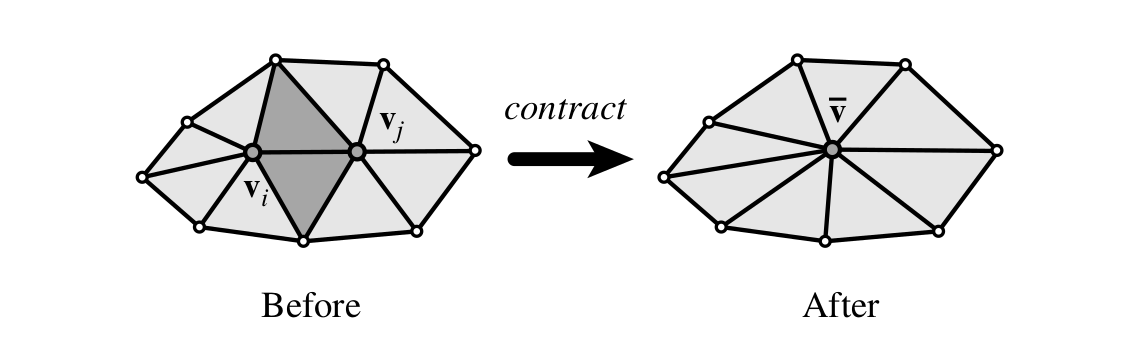
\includegraphics[width=17cm]{edge_contraction}
    \caption{Contraction of an edge \cite{garland99}.}
    \label{fig:edge_contraction_ref}
  \end{center}
\end{figure}

In the parallel framework the crucial aspect is locking all vertices and faces for the current edge to prevent from multiple threads modify the same region. To achieve this, $tryLock()$ method was used. To perform a contraction we have to check if it is possible to lock the whole neighbourhood, in the other case, it means that already a different thread is manipulating a given region. In such a situation the contraction is stopped for the current thread.

The algorithm is a greedy procedure driven by the cost of contraction \cite{cormen01}. It stops when the current threshold level is reached. To achieve simplification we apply a sequence of edge contraction. Where the sequence is created as follows \cite{garland97}:

\begin{enumerate}
\item Select a set of candidate vertex pairs.
\item Assign a cost of contraction to each candidate.
\item Place all candidates in a heap keyed on cost with the minimum cost pair at the top.
\item Repeat until the desired approximation is reached:
\begin{enumerate}
\item Remove the pair $(\mathbf{v_i}, \mathbf{v_j})$ of least cost from the heap.
\item Contract this pair.
\item Update costs of all candidate pairs involving $\mathbf{v_i}$.
\end{enumerate}
\end{enumerate}

Each edge is associated with a cost of contraction which is basically the amount of error made during deletion of a given pair of vertices. This cost is a key in the minimum heap \cite{cormen01} which is iteratively $pop()$. In each main iteration (steps from 1 to 4) we contract edges up to the current adaptive threshold level. If a current edge's cost is bigger or equal than the acceptable error, the main iteration procedure is stopped and the remaining egdes in the heap are ignored. In a next iteration we rebuild the heap and the error level is slightly increased in such a way that perviously contracted regions are even more simplified. The error calculations are based on a hyperparameter $aggressiveness$ and a current iteration value:
\begin{align}
error(i)=0.000000001*(i+3)^a
\end{align}
where $i$ is the iteration and $a$ is the aggressiveness.

Rebulding heap captures the change of geometry made in a  contraction for the whole mesh. After one contraction we update only first order neighbours of a given vertex. Therefore, we need to rebuild heap to reflect the global change.

\section{Assessing Cost of Contraction}
In this section, I will elaborate how to measure the cost of contraction for an edge just for geometry attributes. Maintaining high level of details and faithful representation of the original mesh we should reflect the cost in the effect of changing geometry of the surface. Meaning, if the error is small the geometry changes insignificantly. An edge with a small error is a perfect candiate for removal.

Because the metric is plane-based, first, let me define a standard representation of a plane as $\mathbf{n}^T\mathbf{v}+d=0$ where $\mathbf{n} = [a\;b\;c]^T$, $d$ is a scalar constant and $\mathbf{v} = [x\;y\;z]^T$. From this, we can formulate quadric error metric as following \cite{garland99}:
\begin{align}
D^2(\mathbf{v}) = (\mathbf{n}^T\mathbf{v}+d)^2 = (ax + by + cz + d)^2
\label{quadric_distance}
\end{align}
The error for the set of planes associated with the vertex $v$ is then defiend as (we have to remember that this set is purely conceptual):
\begin{align}
\sum_{i} D_i^2(\mathbf{v}) = \sum_{i} (\mathbf{n_i}^T\mathbf{v}+d_i)^2
\end{align}
Each vertex has accumulated error metric value for surrounding faces  which represents maximum squared distance to the intersection of all planes spanned by each face.

Figure~\ref{fig:measuring_contraction_ref} shows how finding an optimal point $\bar{\mathbf{v}}$ could look in practice in 2D. Vertices $\mathbf{v}_i, \mathbf{v}_j$ define set of planes $P_i = \{A,C\}$ and $P_j = \{B, C\}$. The error on each of those vertices equals $E_{plane}(v_i) = E_{plane}(v_j) = 0$ since they both lie on the lines span by thier sets. Let me define a new set which is a union of $ \bar{P} = P_i \cup P_j = \{ A,B,C \}$. Position of $\bar{\mathbf{v}}$ minimizes the sum of square distances the the lines in $\bar{P}$ \cite{garland99}.

\begin{figure}[H]
  \begin{center}
    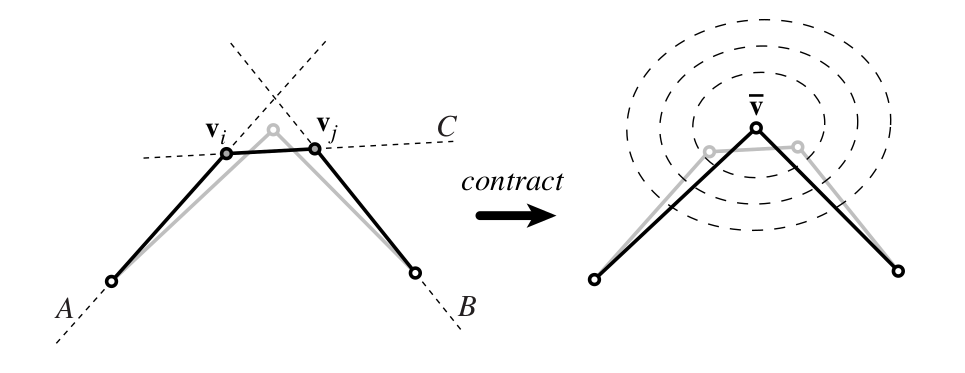
\includegraphics[width=15cm]{measuring_contraction}
    \caption{Measuring contraction cost in 2D \cite{garland99}.}
    \label{fig:measuring_contraction_ref}
  \end{center}
\end{figure}

\section{Quadric Error Metric}

In this section I will introduce the compact representation of the quadric error. First, let me expand the previously declared quadric distance $D^2(\mathbf{v})$~\ref{quadric_distance}.
\begin{align}
D^2(\mathbf{v})&=(\mathbf{n}^T\mathbf{v}+d)^2\\
	  &=(\mathbf{n}^T\mathbf{v}+d)(\mathbf{n}^T\mathbf{v}+d)\\
	  &=(\mathbf{v}^T\mathbf{n}\mathbf{n}^T\mathbf{v}+2d\mathbf{n}^T\mathbf{v}+d^2)\\
	  &=(\mathbf{v}^T(\mathbf{n}\mathbf{n}^T)\mathbf{v}+2(d\mathbf{n})^T\mathbf{v}+d^2)
	  \label{quadric_equation}
\end{align}
where $\mathbf{n}\mathbf{n}^T$ is the outer prodcut of
\begin{align}
\left[
\begin{array}{rrrr}
a^2 & ab & ac   \\
ab  & b^2 & bc  \\
ac  & bc  & c^2 \\
\end{array}\right]
\end{align}
Therefore, the $quadric\;Q$ is defined as a tripe:
\begin{align}
Q = (\mathbf{A},\mathbf{b},c)
\end{align}
Where $\mathbf{A}$ is a $3x3$ matrix, $\mathbf{b}$ is a 3-vector and c is a scalar. We can now rewrite the~\ref{quadric_equation} equation to:
\begin{align}
Q(\mathbf{v}) = \mathbf{v}^T\mathbf{A}\mathbf{v} + 2\mathbf{b}^T\mathbf{v} + c
\end{align}
Quadrics provide an intuitive addition operation which is component-wise: $Q_i(\mathbf{v}) + Q_j(\mathbf{v}) = (Q_i + Q_j)(\mathbf{v})$ where $Q_i(\mathbf{v}) + Q_j(\mathbf{v}) = (\mathbf{A_i} + \mathbf{A_j}, \mathbf{b_i} + \mathbf{b_j}, c_i + c_j)$. Using this fact we can easily define a single quadric $E_Q$ for the set of planes of a given vertex \cite{garland99} as sum over qudrics for each face:
\begin{align}
E_Q(\mathbf{v}) = \sum_{i} D_i^2(\mathbf{v}) = \sum_{i} Q_i(\mathbf{v}) = Q(\mathbf{v})
\end{align}
In other words, each vertex contains accumulated information about the error for the whole local neighbourhood of $\mathbf{v}$. For the pair of vertices the cost of contraction $(\mathbf{v_i}, \mathbf{v_j})\rightarrow\bar{\mathbf{v}}$ is simply:
\begin{align}
Q(\mathbf{\bar{v}}) = Q_i(\mathbf{\bar{v}}) + Q_j(\mathbf{\bar{v}})
\end{align}
The value of $Q(\mathbf{\bar{v}})$ is a key in the min-heap. Tables~\ref{tab:approx_bunny_ref} and~\ref{tab:wireframe_ref} show an example of simplification using quadric metric. Due to complexity of the original Stanford Bunny mesh which has 69451 faces, I first simplified it to 3642 faces and used this as a reference model.

\begin{table}[h!]
\centering
\begin{tabular}{ |c|c| } 
 \hline
 Number of faces & Original simplification\\
 \hline
 3642 faces & 94.756 \\ 
 2228 faces & 96.791 \\ 
 1842 faces & 97.347\\ 
 1152 faces & 98.341\\ 
 665 faces & 99.042\\ 
 130 faces & 99.813\\
 \hline
\end{tabular}
\caption{Percentage of simplification of the original Stanford Bunny with 69351 faces.}
\end{table}
Table~\ref{tab:original_ref} shows the quality of progressive simplification. As you can see, 70\% of reduction is hard to distinguish from the original mesh, even the 94\% is still a good approximation and features of the bunny are preserved fairly well.

\begin{center}
  	\begin{table}[H]
  	\begin{center}
  	\begin{tabular}{cc}
	\begin{subfigure}{0.7\textwidth}\centering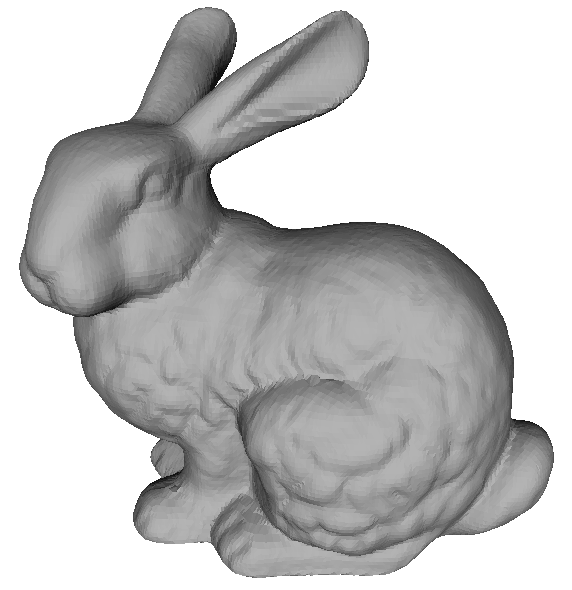
\includegraphics
		[width=0.5\columnwidth]{original_100}\caption{Faces 69451 (100\%)}\label{original_100_ref}\end{subfigure}\\
	\begin{subfigure}{0.7\textwidth}\centering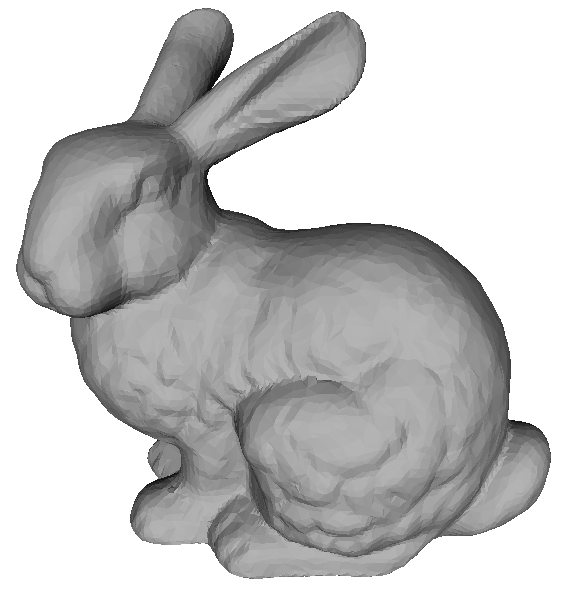
\includegraphics
		[width=0.5\columnwidth]{original_70}\caption{Faces 18892 (30\%)}\label{original_70_ref}\end{subfigure}\\
	\begin{subfigure}{0.7\textwidth}\centering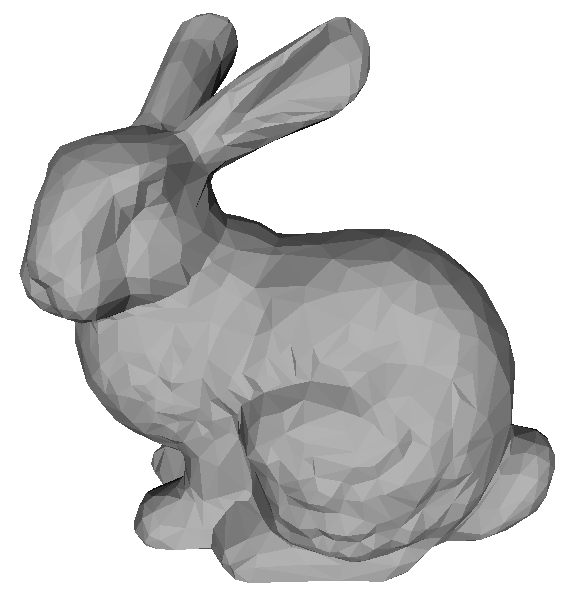
\includegraphics
		[width=0.5\columnwidth]{original_95}\caption{Faces 3642 (6\%)}\label{original_95_ref}\end{subfigure}\\
	\end{tabular}
	\caption{Quality of the simplification of the original mesh.}
  	\label{tab:original_ref}
  	\end{center}
	\end{table}
\end{center}

\begin{center}
  	\begin{table}[H]
  	\begin{center}
  	\begin{tabular}{cc}
	\begin{subfigure}{0.4\textwidth}\centering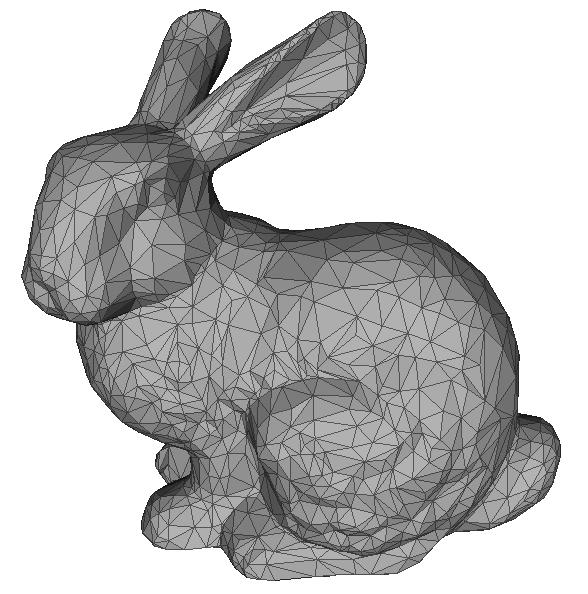
\includegraphics
		[width=0.7\columnwidth]{bunny_100}\caption{Faces 3642}\label{ref_label1}\end{subfigure}&	
	\begin{subfigure}{0.4\textwidth}\centering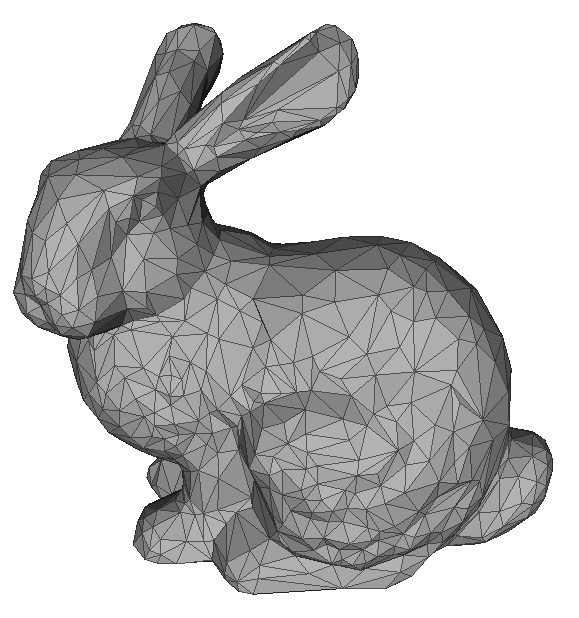
\includegraphics
		[width=0.7\columnwidth]{bunny_80}\caption{Faces 2228}\label{bunny_80_ref}\end{subfigure}\\
	\newline
	\begin{subfigure}{0.4\textwidth}\centering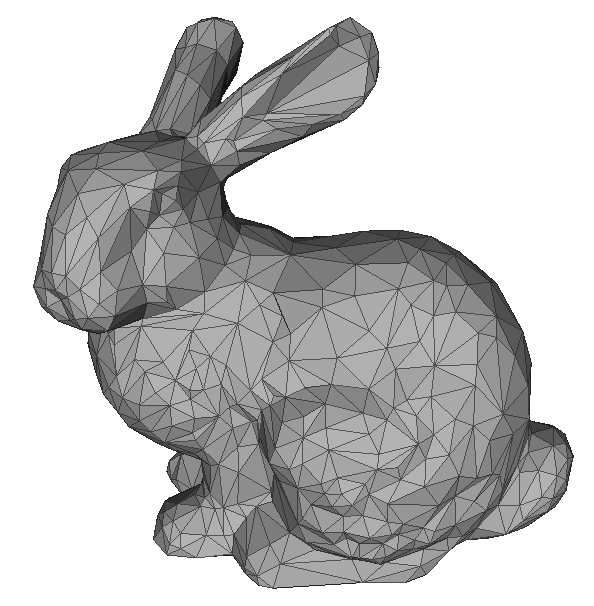
\includegraphics
		[width=0.7\columnwidth]{bunny_70}\caption{Faces 1842}\label{bunny_70_ref}\end{subfigure}&
	\begin{subfigure}{0.4\textwidth}\centering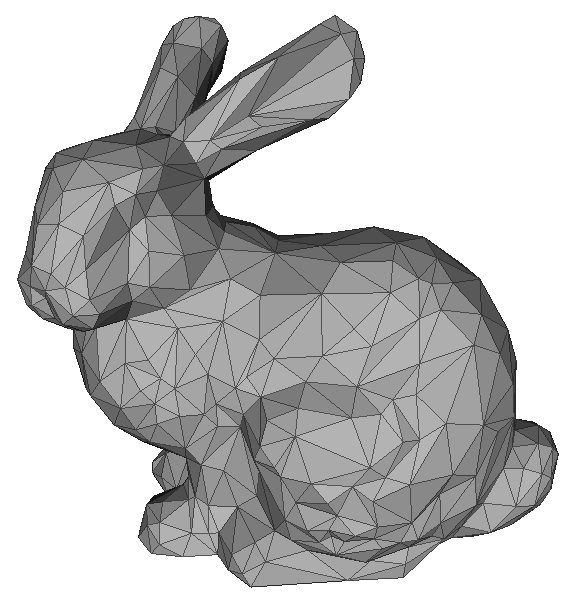
\includegraphics
		[width=0.7\columnwidth]{bunny_60}\caption{Faces 1152}\label{bunny_60_ref}\end{subfigure}\\
	\newline
	\begin{subfigure}{0.4\textwidth}\centering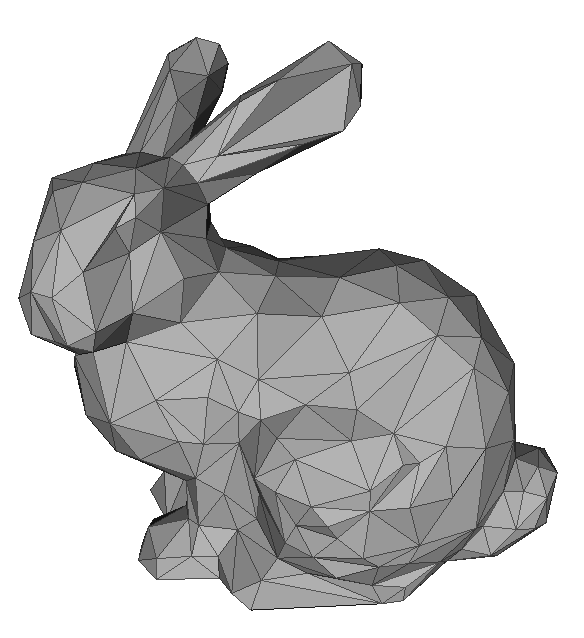
\includegraphics
		[width=0.7\columnwidth]{bunny_50}\caption{Faces 655}\label{bunny_50_ref}\end{subfigure}&
	\begin{subfigure}{0.4\textwidth}\centering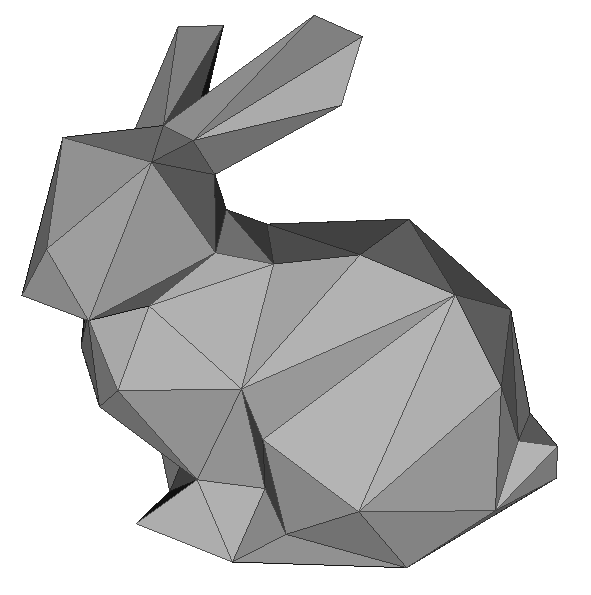
\includegraphics
		[width=0.7\columnwidth]{bunny_40}\caption{Faces 130}\label{bunny_40_ref}\end{subfigure}\\
	\end{tabular}
  	\caption{Several approximations of Stanford Bunny constructed with the geometry quadric error metric.} \label{tab:approx_bunny_ref}
  	\end{center}
	\end{table}
\end{center}

\begin{center}
  	\begin{table}[H]
  	\begin{center}
  	\begin{tabular}{cc}
	\begin{subfigure}{0.4\textwidth}\centering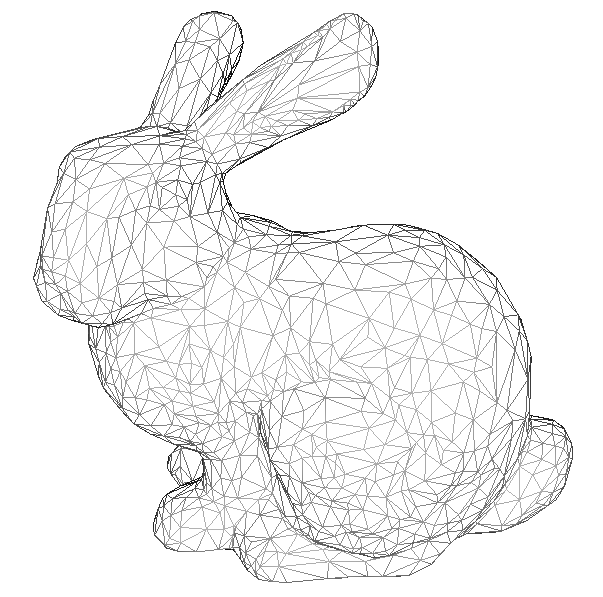
\includegraphics
		[width=0.7\columnwidth]{wireframe_100}\caption{Faces 3642}\label{wireframe_100_ref}\end{subfigure}&	
	\begin{subfigure}{0.4\textwidth}\centering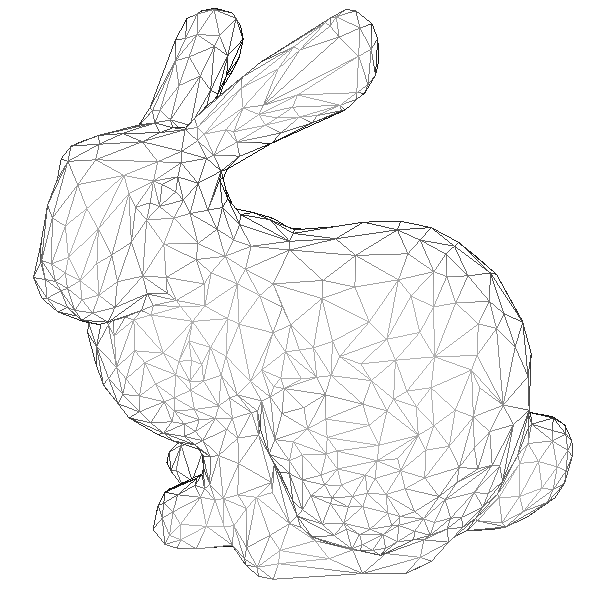
\includegraphics
		[width=0.7\columnwidth]{wireframe_80}\caption{Faces 2228}\label{wireframe_80_ref}\end{subfigure}\\
	\newline
	\begin{subfigure}{0.4\textwidth}\centering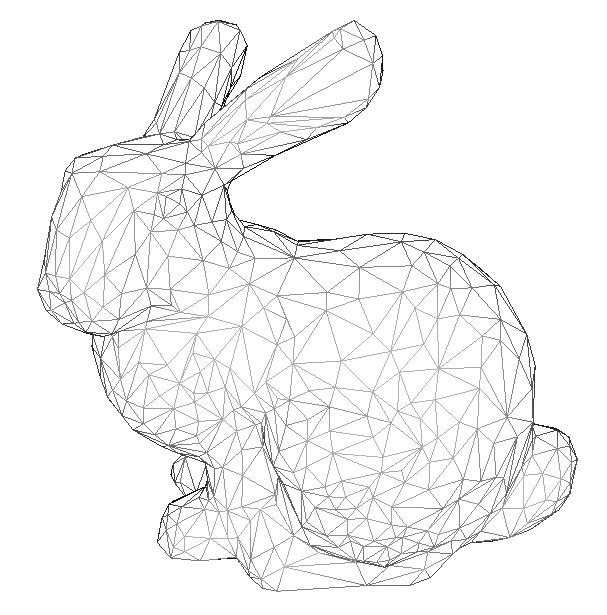
\includegraphics
		[width=0.7\columnwidth]{wireframe_70}\caption{Faces 1842}\label{wireframe_70_ref}\end{subfigure}&
	\begin{subfigure}{0.4\textwidth}\centering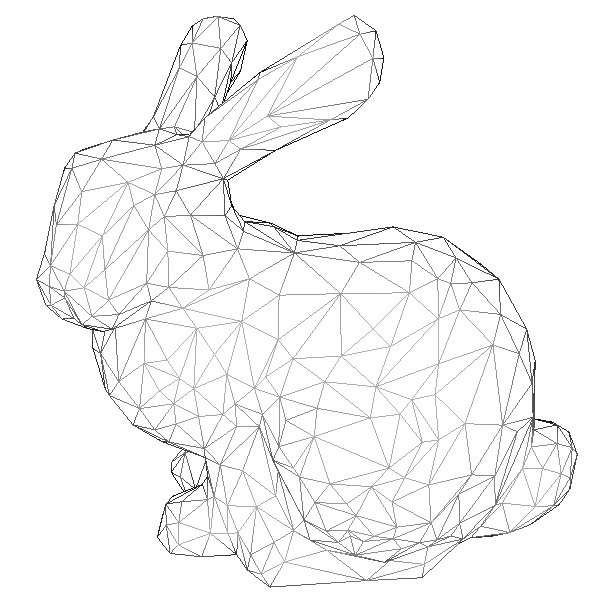
\includegraphics
		[width=0.7\columnwidth]{wireframe_60}\caption{Faces 1152}\label{wireframe_60_ref}\end{subfigure}\\
	\newline
	\begin{subfigure}{0.4\textwidth}\centering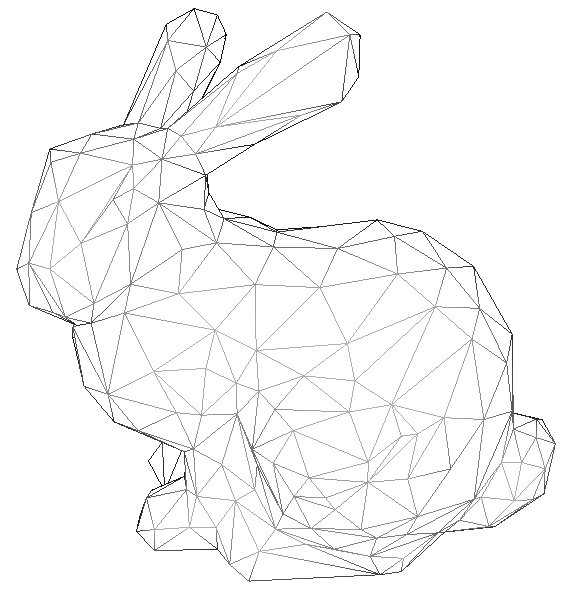
\includegraphics
		[width=0.7\columnwidth]{wireframe_50}\caption{Faces 655}\label{wireframe_50_ref}\end{subfigure}&
	\begin{subfigure}{0.4\textwidth}\centering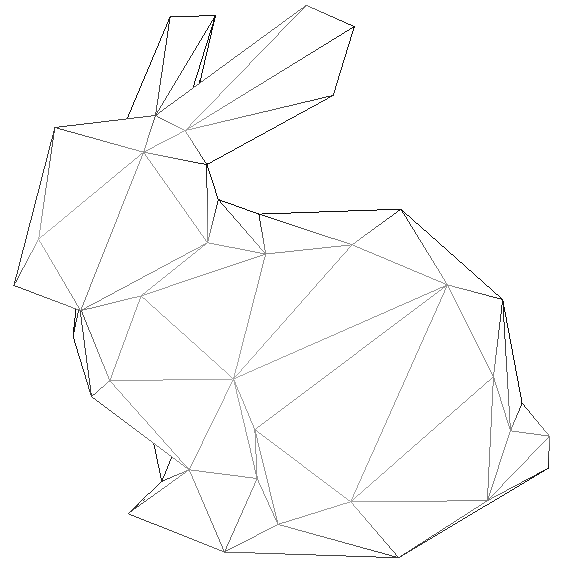
\includegraphics
		[width=0.7\columnwidth]{wireframe_40}\caption{Faces 130}\label{wireframe_40_ref}\end{subfigure}\\
	\end{tabular}
  	\caption{Wireframe versions of models in Table~\ref{tab:approx_bunny_ref}}
  	\label{tab:wireframe_ref}
  	\end{center}
	\end{table}
\end{center}

\newpage
\section{Vertex Placement}

To perform the contraction of an edge $(\mathbf{v_i}, \mathbf{v_j})\rightarrow\bar{\mathbf{v}}$ we have to calcualte a new position of $\mathbf{\bar{v}}$ which is called the target. The optimal placement strategy, therefore, is to find a point for which $Q(\mathbf{\bar{v}})$ is minimal. Fortunately, since, $Q(\mathbf{\bar{v}})$ is quadratic we are guaranteed to find an unique minimizer which is a global minimum.
\begin{align}
Q(\mathbf{v}) &= \mathbf{v}^T\mathbf{A}\mathbf{v} + 2\mathbf{b}^T\mathbf{v} + c\\
\nabla Q(\mathbf{v}) &= 2\mathbf{A}\mathbf{v} + 2 \mathbf{b}
\end{align}
Solving for $\nabla Q(\mathbf{v}) = 0$, the optimal position is defined:
\begin{align}
\mathbf{\bar{v}} = -\mathbf{A}^{-1}\mathbf{b}
\end{align}
and the error:
\begin{align}
Q(\mathbf{\bar{v}}) = \mathbf{b}^T\mathbf{\bar{v}} + c = -\mathbf{b}^T\mathbf{A}^{-1}\mathbf{b} + c
\end{align}

The function used to calculate the optimal position $\mathbf{\bar{v}}$ is the following:
\begin{center}
\begin{lstlisting}[caption={LU decomposition for solving a linear system.},captionpos=b]
virtual bool optimize(Eigen::VectorXd &result) {
	Eigen::FullPivLU<Eigen::MatrixXd> lu = A.fullPivLu();
	if (!lu.isInvertible())
		return false;
	result = -lu.solve(b);
	return true;
};
\end{lstlisting}
\end{center}
Eigen::FullPivLU is LU decomposition of a matrix with complete pivoting, and related features. This decomposition provides the generic approach to solving systems of linear equations, computing the rank, invertibility, inverse, kernel, and determinant \cite{eigenLU19}.

In the case when a matrix is not invertible the following computations are performed \cite{garland99}:
\begin{enumerate}
\item If $\mathbf{A}$ is singular, find the optimal position along the line segment $(\mathbf{v_i}, \mathbf{v_j})$.
\item If this is not unique, select the better of $\mathbf{v_i}$ and $ \mathbf{v_j}$.
\end{enumerate}
In practice it is very rare that a matrix determinant is zero. Due to the limits of floating point precision. The optimal vertex placement will tend to create closely fitting approximations of the original mesh. Which at the end gives a better shaped triangles \cite{garland99}. The placement strategy for the pair of contraction $(\mathbf{v_i}, \mathbf{v_j})$ is to always move $\mathbf{v_j}$ to the position of $\mathbf{v_i}$. It eliminates a problem of storing delta of the new vertex position.

\newpage
\section{Constraints}

Simplification requiers several different constrains and checks to not introduce an error in the new vertex placement position. The quality of approximation is critical for producing simplified meshes. For instance, the borders of a mesh have to be treated as a special case.

There is a few options how we can solve the problem of borders. In my implementation, I used a version with adding the quadric error of a plane perpendicular to a given border edge. The perpendicular plane itself defines a boundary constraint. The other option is to do not touch border vertices. However, this option is problematic if we want to achieve a certain level of simplification. The number of border vertices can be even 15\% of the mesh. It means that this 15\% has to be transferd from the complex shapes which we would like to preserve to the simplification pool. Therefore, we sacrifice the quality of the mesh for the sake of preserving edges.

\begin{figure}[h!]
  \begin{center}
    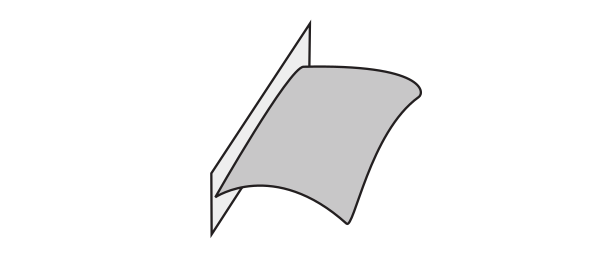
\includegraphics[width=13cm]{border_constraint}
    \caption{An example of the border constrain \cite{garland99}.}
    \label{fig:border_constraint}
  \end{center}
\end{figure}

The perpendicular plane constraint is very convinient in many aspects. For instance, it requires only to calculate the quadric error and add this error to the initial quadric error of each vertex on the boundary. It can be easily done in the initalization step when the heap is built. After each main iteration, the vertices are flagged if they lay on the border. Once the perpendicular error planes are accumulated in the vertices the algorithm continues the regular routine.

We can additionally weight the perpendicular plane constraint by an arbitrary factor. I do not use the factor multiplication because of the adaptive thresholding, which ignores all edges above the current threshold level. In my version of the algorithm, the edges are consumed as soon as possible to reduce the simplification pool.

The other very important problem is vertex folding. A vertex placement can introduce a new position for a vertex which folds the neighbourhood and procudes degeneracies into the mesh. 

\begin{figure}[H]
  \begin{center}
    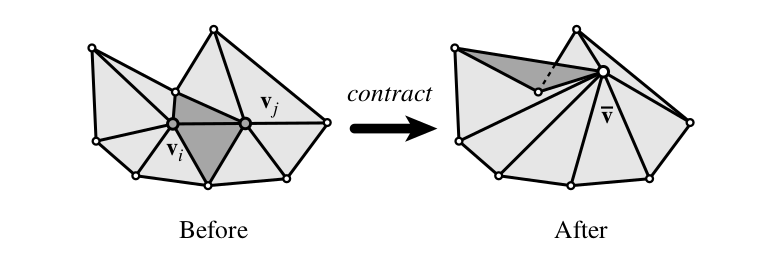
\includegraphics[width=15cm]{fold}
    \caption{An edge contraction which causes the mesh to fold over on itself \cite{garland99}.}
    \label{fig:fold}
  \end{center}
\end{figure}

Before performing a contraction the algorithm has to check if the new position is a valid one. For example Figure \ref{fig:fold} shows that the new position $\mathbf{\bar{v}}$ is degenerated and it folds one of the faces into the darkened area. In this case we have to stop contraction for this particular edge. To detect those kind of situations I examine the normals of the faces around $\mathbf{v_i}, \mathbf{v_j}$. If the face normal changes by some threshold level, the contraction is assumed to introduce flipping and is discarded.

\newpage
\section{Summary of Garland's Algorithm}

Below, I present the complete algorithm in 5 steps. In the next chapter I will elaborate how this concept is incorporated in multithreded approach.

Algorithm \cite{garland99}:

\begin{enumerate}
\item Select a set of candidate vertex pairs $(\mathbf{v_i}, \mathbf{v_j})$.
\item Allocate a quadric $Q_i$ for each vertex $\mathbf{v_i}$.
\item For each face compute a quadric $Q_i$. Add this fundamental quadric to the vertex quadrics $Q_i, Q_k, Q_l$ and optionaly weight it appropriately.
\item For each candidate pair $(\mathbf{v_i}, \mathbf{v_j})$:
\begin{enumerate}
\item Compute $Q = Q_i + Q_j$.
\item Select a target position $\mathbf{\bar{v}}$.
\item Apply consistency checks and penalties.
\item Place pair in heap keys on cost $Q(\mathbf{\bar{v}})$
\end{enumerate}
\item Repeat unitl the desired approximation is reached:
\begin{enumerate}
\item Remove the pair $(\mathbf{v_i}, \mathbf{v_j})$ of least cost from the heap.
\item Preform contraction $(\mathbf{v_i}, \mathbf{v_j})\rightarrow\bar{\mathbf{v}}$
\item Set $Q_i = Q_i + Q_j$.
\item For each remaining pair $(\mathbf{v_i}, \mathbf{v_j})$, compute target position and cost as in step 4; update heap.
\end{enumerate}
\end{enumerate}

The above algorithm is the main core of my implemenation. Every thread will perform the simplification using quadric error metrics, based on Garland's work. In the next chapter, I would like to give a brief introduction to the extended version of the algoritm which includes color and normals.

\chapter{Extended Simplification Algorithm}

The previous implementation includes only geometric error. In this chapter we incorporate more attributes to improve simplification. Using additionally, color and normals we can easier deceminate planar surfaces and achieve better results. However, in the noisy environment of color (which is usually the case in scans), gradient guided simplification may produce poor results.

\section{Design}
In this section we assume that each vertex is additionally associated with color $\mathbf{c} = [r \ g \ b]^T$ and $\mathbf{n} = [nx \ ny \ nz]^T$. For the sake of simplicity, lets consider an example with geometry and color only. Assume that each vertex is attributed with $\mathbf{v} = [x \ y \ z \ r \ g \ b]^T$. Figure~\ref{fig:hexagon} shows an example of such a mesh. A triangle is defined as $T = (\mathbf{p}, \mathbf{q}, \mathbf{r})$ with edges $\mathbf{h} = \mathbf{q} - \mathbf{p}$ and $\mathbf{k} = \mathbf{r} - \mathbf{p}$. Now, because our problem is more that 3 dimensional, we have to use a different method to calucalte orthogonal vectors to the plane defined by the face, than simply calculating a corss product. Fortunately, Gram-Schmidt orthogonalization \cite{strang88} helps us to solve this problem.

\begin{figure}[H]
  \begin{center}
    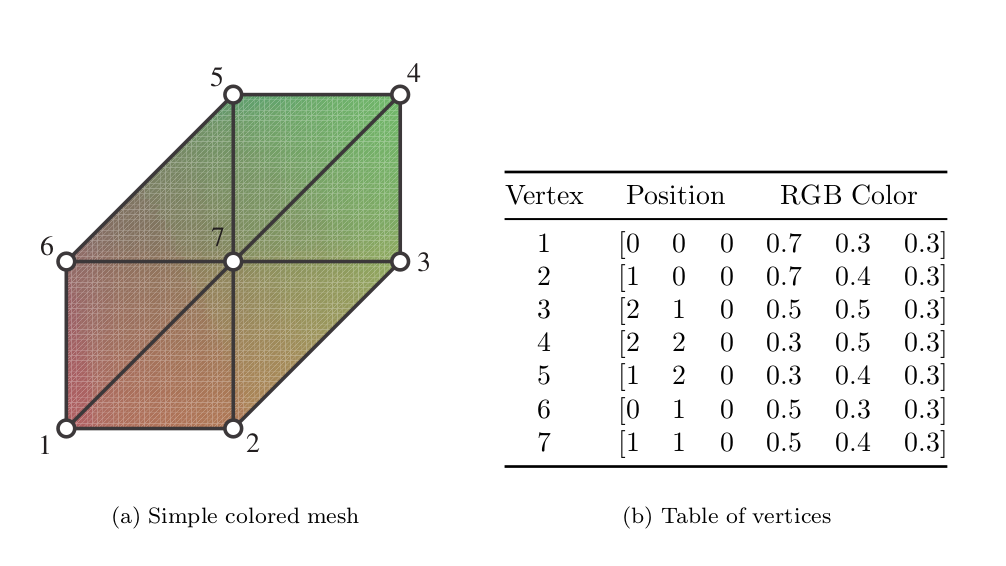
\includegraphics[width=15cm]{hexagon}
    \caption{A triangulated hexagon with color values at each vertex \cite{garland99}.}
    \label{fig:hexagon}
  \end{center}
\end{figure}

We have to find 2 vectors $\mathbf{e_1}, \mathbf{e_2}$ which are orthogonal to each other.

\begin{align}
\mathbf{e_1} &= \mathbf{h} / \norm{\mathbf{e_1}} \\
\mathbf{e_2} &= \frac{\mathbf{k} - (\mathbf{e_1} \cdot \mathbf{k})\mathbf{e_1}}{\norm{\mathbf{k} - (\mathbf{e_1} \cdot \mathbf{k})\mathbf{e_1}}}
\end{align}

Those equations give us 2 unit-length vectors which form a local coordinate system with $\mathbf{p}$ as the origin.

\begin{figure}[H]
  \begin{center}
    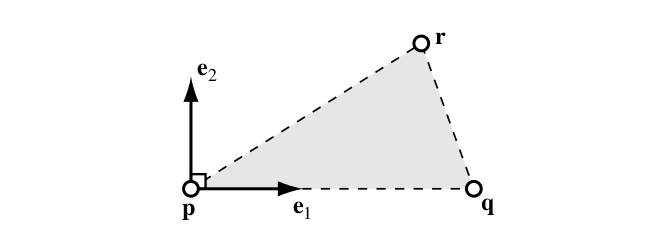
\includegraphics[width=12cm]{gram}
    \caption{Orthonomal vectors \cite{garland99}.}
    \label{fig:gram}
  \end{center}
\end{figure}

Let me define a distance from an arbitrary point $\mathbf{v}\in\mathbf{R}^n$ to the plane created by the face $T$. The squared distance of the vector $\mathbf{u} = \mathbf{p} - \mathbf{v}$ is defined as \cite{garland99}

\begin{align}
\norm{\mathbf{u}}^2 = \mathbf{u}^T\mathbf{u} = (\mathbf{u}^T\mathbf{e_1})^2 + ... +  (\mathbf{u}^T\mathbf{e_n})^2
\end{align}

We can rearrange this equation to:

\begin{align}
(\mathbf{u}^T\mathbf{e_3})^2 + ... +  (\mathbf{u}^T\mathbf{e_n})^2 = \norm{\mathbf{u}}^2 - (\mathbf{u}^T\mathbf{e_1})^2 - (\mathbf{u}^T\mathbf{e_2})^2
\end{align}

The left hand side is the squared distance of $\mathbf{u}$ along all the axes perpendicular to the plane of $T$. This is a distance between this vector $\mathbf{v}$ and the plane $T$.

\begin{align}
D^2 = \mathbf{u}^T\mathbf{u} - (\mathbf{u}^T\mathbf{e_1})(\mathbf{u}^T\mathbf{e_1}) - (\mathbf{u}^T\mathbf{e_2})(\mathbf{u}^T\mathbf{e_2})
\end{align}

The quadric metric is defined then as $Q(\mathbf{v}) = \mathbf{v}^T\mathbf{A}\mathbf{v} + 2\mathbf{b}^T\mathbf{v} + c$ where:

\begin{align}
\mathbf{A} &= \mathbf{I} - \mathbf{e_1}\mathbf{e_1}^T - \mathbf{e_2}\mathbf{e_2}^T\\
\mathbf{b} &= (\mathbf{p} \cdot \mathbf{e_1})\mathbf{e_1} + (\mathbf{p} \cdot \mathbf{e_2})\mathbf{e_2} - \mathbf{p}\\ 
\mathbf{c} &= \mathbf{p} \cdot \mathbf{p} - (\mathbf{p} \cdot \mathbf{e_1})^2 - (\mathbf{p} \cdot \mathbf{e_2})^2 
\end{align}

The matrix $\mathbf{A}$ from \ref{fig:hexagon} is then:

\begin{align}
\left[
\begin{array}{rrrrrr}
0.06 & 0 & 0 & 0 & -0.59 & 0\\
0 & 0.23 & 0 & 1.15 & 0 & 0\\
0 & 0 & 6.00 & 0 & 0 & 0\\
0 & 1.15 & 0 & 5.77 & 0 & 0\\
-0.59 & 0 & 0 & 0 & 5.94 & 0\\
0 & 0 & 0 & 0 & 0 & 6.00
\end{array}\right]
\end{align}

Building the quadric and finding the optimal position is exactly the same like in the geometry case. To use different metric we have to only change computations of orthonormal vectors.

\begin{figure}[H]
  \begin{center}
    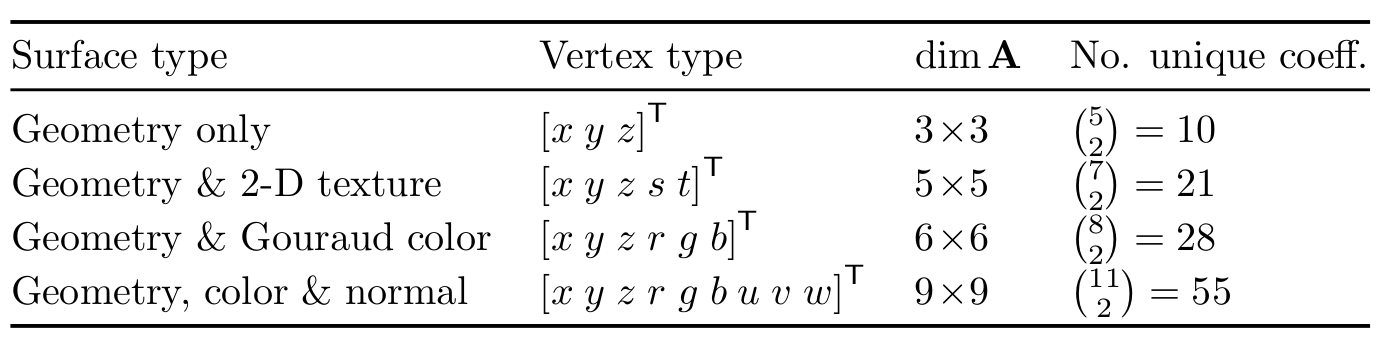
\includegraphics[width=15cm]{params_table}
    \caption{Summary of common extended quadric types \cite{garland99}.}
    \label{fig:params_table}
  \end{center}
\end{figure}

\section{Results}

Table \ref{tab:color_simplification} shows the results of using color and geometry metric error. We can easily notice that the simplifcation follows the color pattern. In some cases its a desired features, however, we have to be careful about the noise of the gradient.

In the case of 3D scanning we get vertices with several attributes; for instance color, normal and geometry. Unfortunately, the color introduces quite substantial error. If the color gradient was constant in most of the places, the whole simplification would hugely benefit from it. However, not only a camera introduces an error but also a SLAM algorithm. Therefore, we either incorporate, normals, color, geometry all together or use them separately.

As you can see in the Table \ref{tab:desk}, complex shapes like plants or a small fan in front of the monitor preserve their initial complexity. However, flat surfaces like the desk or the monitor are significally simplified. Therefore, the amount of removable faces, to achieve a particular simplification level, was transfered from the complex shapes pool to the flat surface pool. Complex shapes will be simplified only in the case when planar surfaces are as simply as possbile and removal is not longer available.

\begin{center}
  	\begin{table}[H]
  	\begin{center}
  	\begin{tabular}{cc}
	\begin{subfigure}{0.8\textwidth}\centering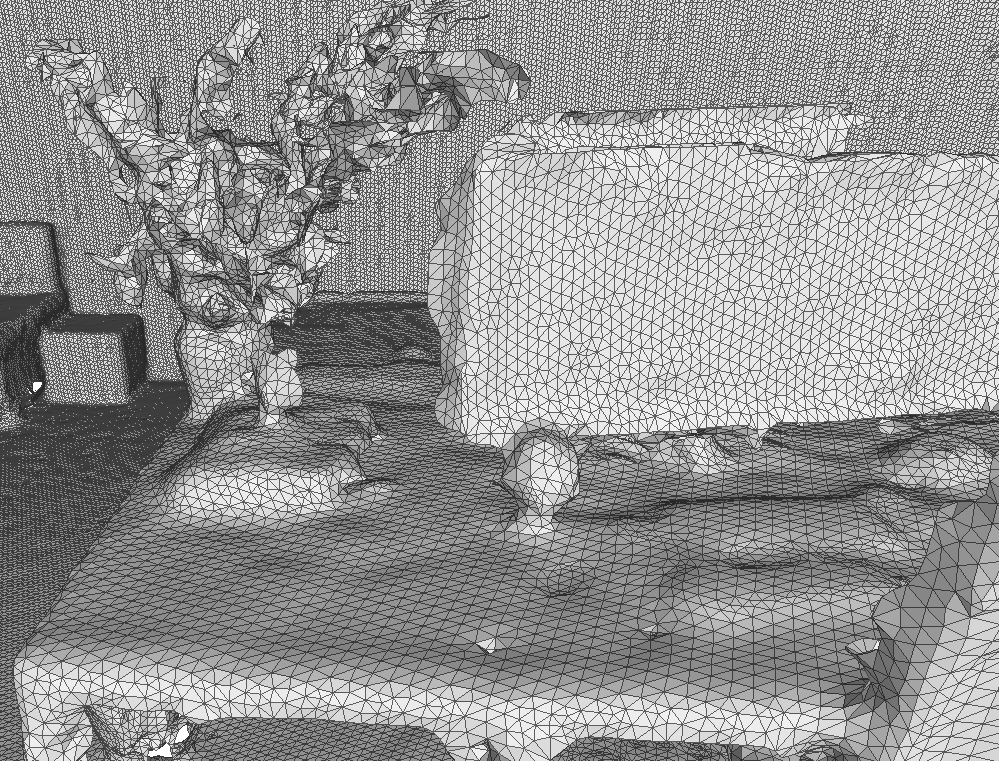
\includegraphics
		[width=1\columnwidth]{desk_2}\caption{Original}\label{original_100_ref}\end{subfigure}\\
	\begin{subfigure}{0.8\textwidth}\centering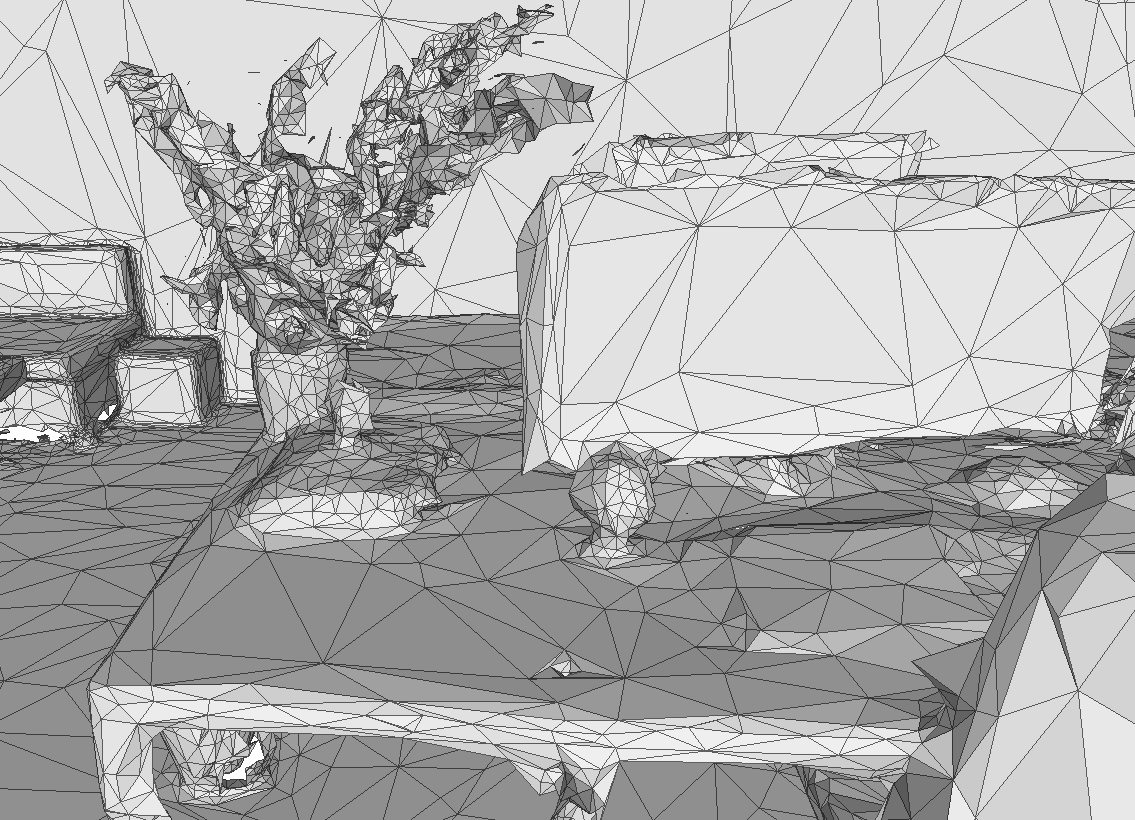
\includegraphics
		[width=1\columnwidth]{desk}\caption{Color, geometry and normal simplification}\label{original_70_ref}\end{subfigure}\\
	\end{tabular}
	\caption{Comparison of simplification with all attributes [geometry, color, normal] with 87\% of reduction to the original mesh.}
  	\label{tab:desk}
  	\end{center}
	\end{table}
\end{center}

\newpage
\begin{center}
  	\begin{table}[H]
  	\begin{center}
  	\begin{tabular}{cc}
	\begin{subfigure}{0.5\textwidth}\centering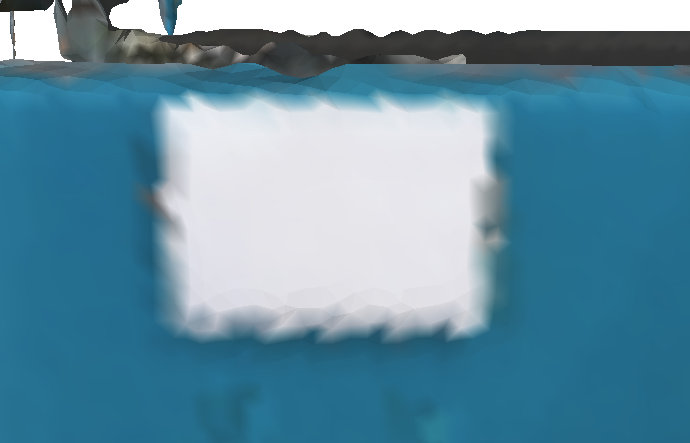
\includegraphics
		[width=8cm,height=6cm]{color_1}\caption{Original}\label{color1}\end{subfigure}&	
	\begin{subfigure}{0.5\textwidth}\centering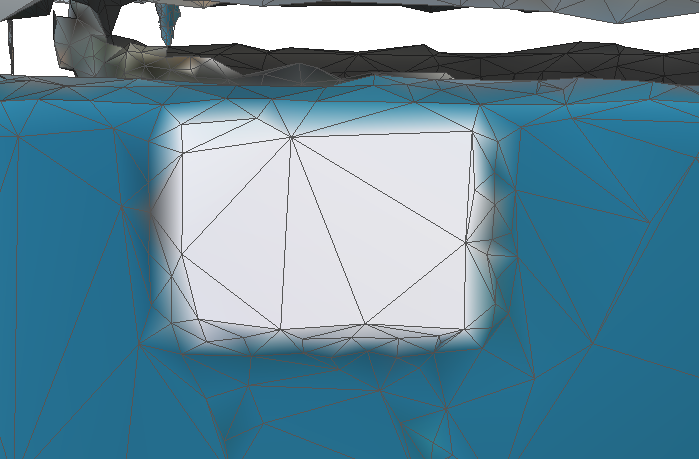
\includegraphics
		[width=8cm,height=6cm]{color_2}\caption{Color and geometry simplification}\label{color2}\end{subfigure}\\
		\newline
			\begin{subfigure}{0.5\textwidth}\centering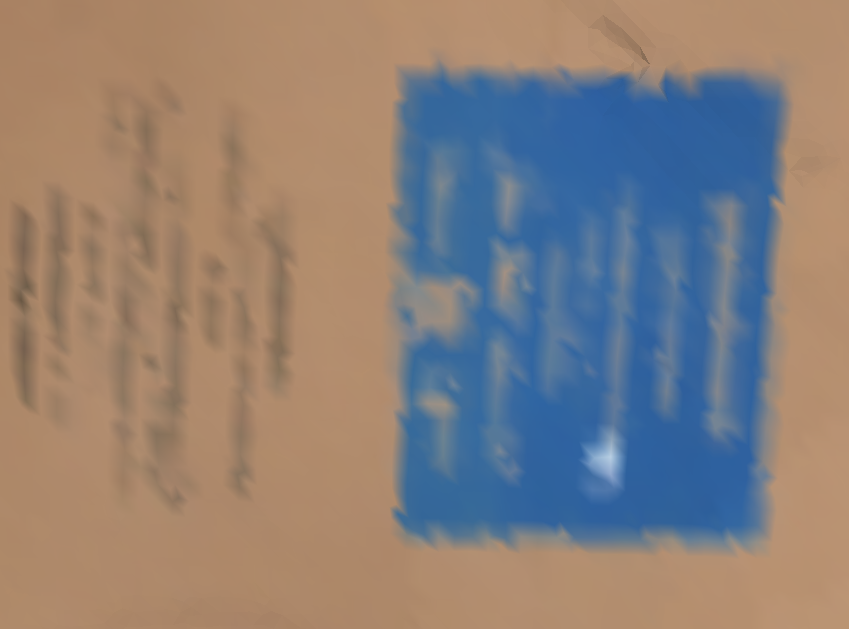
\includegraphics
		[width=8cm,height=6cm]{color_4}\caption{Original}\label{color1}\end{subfigure}&	
	\begin{subfigure}{0.5\textwidth}\centering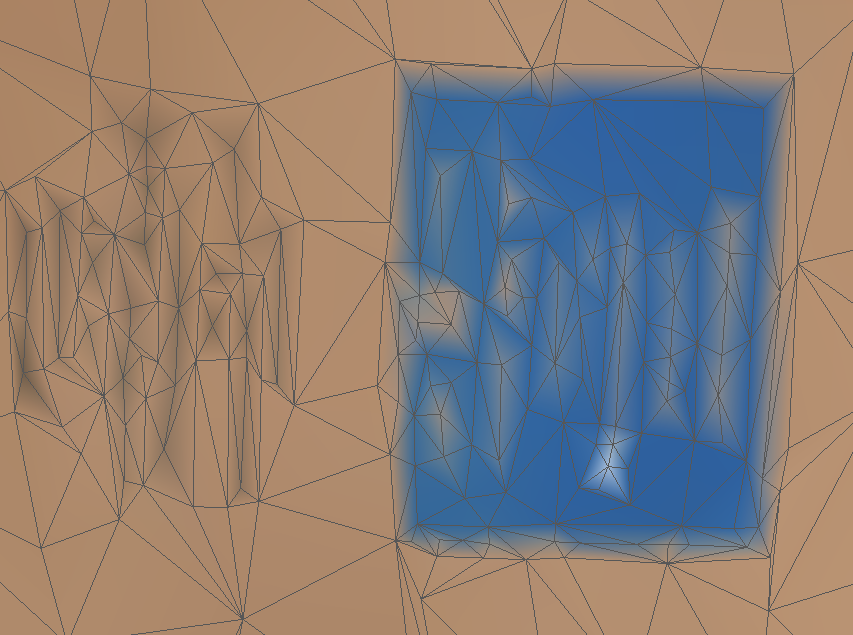
\includegraphics
		[width=8cm,height=6cm]{color_3}\caption{Color and geometry simplification}\label{color2}\end{subfigure}\\
				\newline
			\begin{subfigure}{0.5\textwidth}\centering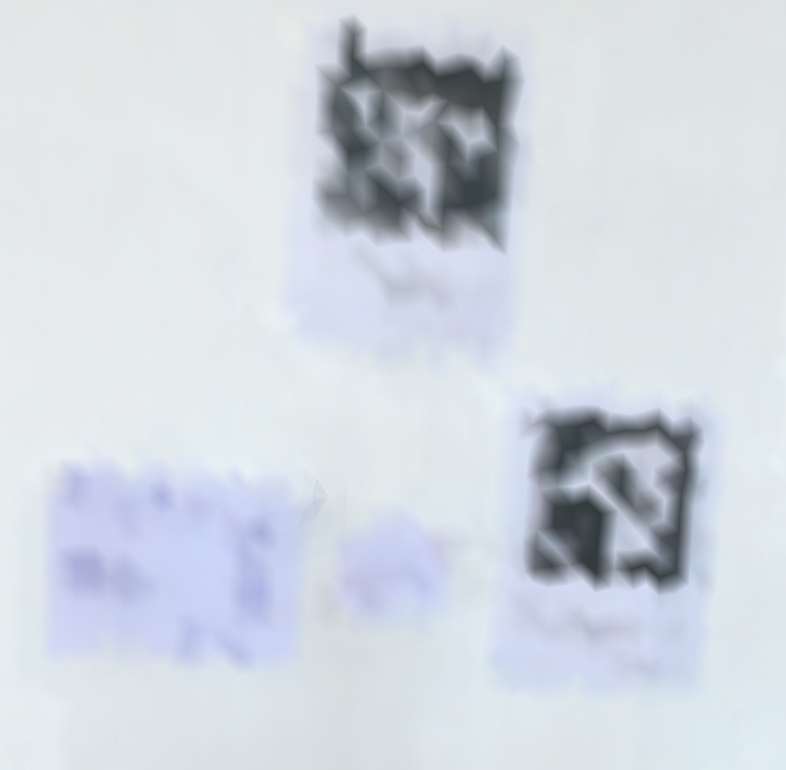
\includegraphics
		[width=8cm,height=6cm]{color_5}\caption{Original}\label{color1}\end{subfigure}&	
	\begin{subfigure}{0.5\textwidth}\centering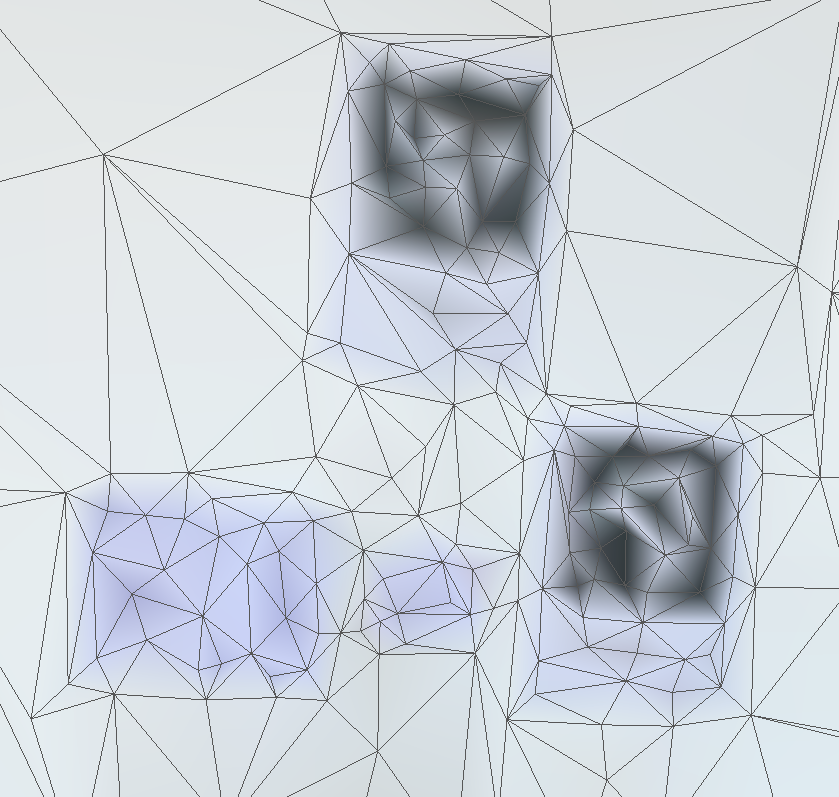
\includegraphics
		[width=8cm,height=6cm]{color_6}\caption{Color and geometry simplification}\label{color2}\end{subfigure}
		\end{tabular}
  	\caption{Comparison of gradient guided simplification [geometry, color].} \label{tab:color_simplification}
  	\end{center}
	\end{table}
\end{center}


\chapter{Parallel Simplification Algorithm}

In this chapter, I will describe my approach to design a parallel version of Garland's simplification algorithm. First, I would like to describe Producer-Consumer design patter, libraries and ideas used in the implementation to make it thread-safe. Next, I will analyze the speedup and potential problems which can arose during an exacution. Finally, summarize the approach and elaborate further improvements.

\section{Producer Consumer Pattern}

The producer-consumer pattern is a perfect way to separate workload of processing data from the work to produce them. In other words, we divide our problem into two major components connected usually by a queue. This is a classic example of a multi-process synchronization problem. The process separation gives us clear view at the problem and tasks. A producer is placing items in a queue, and a consumer removes each task from the queue and processes the data. This decoupling means that two components are completely independent \cite{grand02}. In the case when the queue is full, we usually $spinlock$ producers waiting for consumers to process tasts.

\begin{figure}[H]
  \begin{center}
    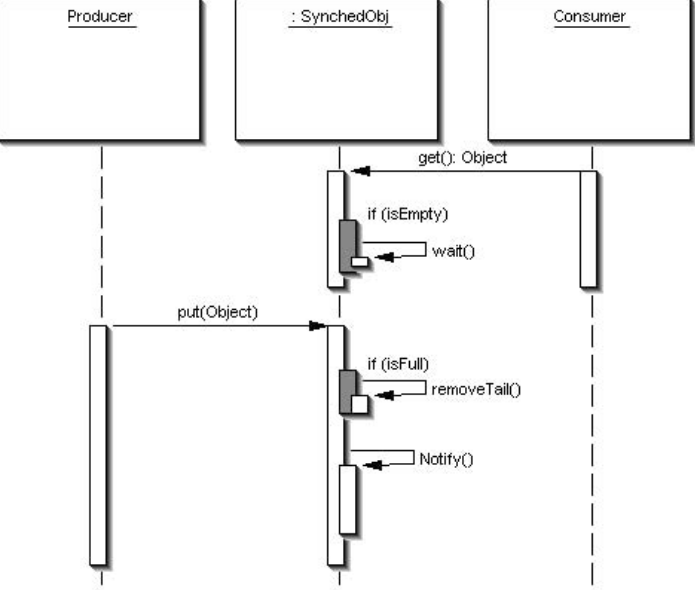
\includegraphics[width=12cm]{producer_consumer}
    \caption{UML sequence diagram for the procuder-consumer pattern implementation.}
    \label{fig:uml}
  \end{center}
\end{figure}

Figure \ref{fig:uml} shows how such a process could look like. We can see 3 main components; producer, synchronization object (the queue) and consumer. In the case when the buffer is either full or empty, we use $spin$ to wait for more tasks or wait for consumer to empty the queue.

In my implementation, I use a generalized version of this patter for multiple procuders and consumers operating on a single fixed buffer. The main idea is to first cluster the mesh to create a separate tasks, which later are consumed by threads from a threadpool.

\newpage
\section{Producer Desing}

To cluster a mesh I use a simple method of dividing the bounding box around the mesh into sub-boxes. When the mesh is read, I calculate the global bounding box, which later is divided into predifined number of clusters.

\begin{figure}[H]
  \begin{center}
    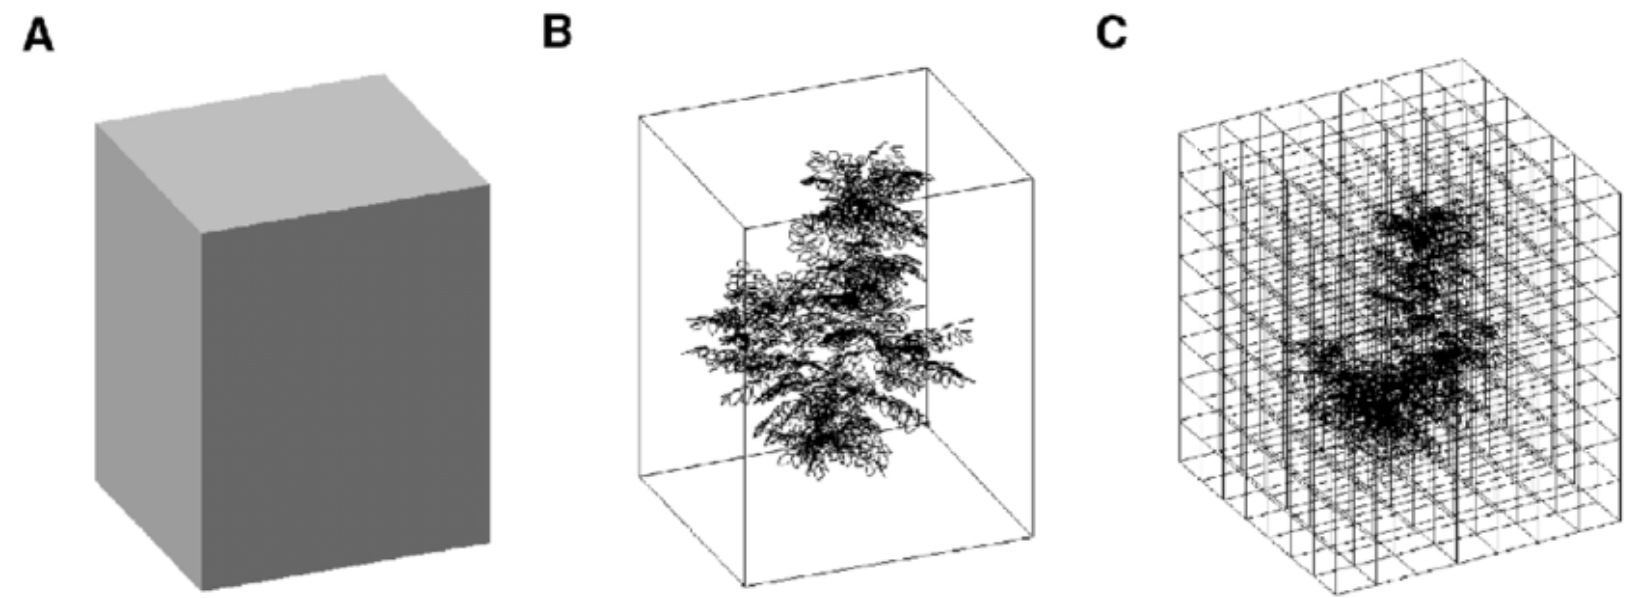
\includegraphics[width=14cm]{clustering}
    \caption{Example of clustring a mesh into 7x7x7 clusters.}
    \label{fig:clustering}
  \end{center}
\end{figure}

Figure\ref{fig:clustering} shows an example with 343 clusters, where each dimention of the main bounding box $[B]$ was divided into 7 equal parts $[C]$. When clausters are calculated we can easily check which face belongs to which cluster. In the case when a face intersects multiple clusters the voting is done. If two vertices of a face belong to the same cluster this box is selected as a holder of the face. If each vertex belongs to a different cluster, randolmy select one box. The pseudocode of the producer is the following:
\newline
\begin{center}
\begin{lstlisting}[caption={C style psuedocode of a producer},captionpos=b]
void function produce {
    clusters = getClusters(size, masterMesh);
    for (cluster : clusters){
        set faceCluster to empty
        for (face : cluster.elements){
            if vote(face) is true
                add face to faceCluster
        }
        add faceCluster to queue
    }
};
\end{lstlisting}
\end{center}

In the line 7 the $vote()$ function is used to assing the correct cluster id and membership of a face. In the line 9 we insert the $faceCluster$ to the queue for further processing.

\newpage
\section{Consumer Desing}

The consumer process is desing in a way to utilize funcionality of $\inlinecode{Java}{boost::thread_group}$ and $\inlinecode{Java}{boost::asio::io_service}$. Thread group is a class which helps with management and provides a container for easy grouping of threads to simplify several common thread creation and management idioms \cite{boost03}. A user has to specify how many threads will be created and added to the threadpool. Those threads operate directly on the queue, removing tasks and processing data. In this case they are preforming simplification of a mesh on each cluster independently.
\newline
\begin{center}
\begin{lstlisting}[caption={C style psuedocode of a task for a consumer},captionpos=b]
void function task {
    garland = QSlim();
    garland->setClustersAABBs();
    garland->initialize<QuadricError>();
    garland->simplify<QuadricError>();
};
\end{lstlisting}
\end{center}

Each task gets a single cluster to process. The $QuadricError$ is a type of a quadric error metric where we specify attributes for the calculations like; geometry, color, normals. The class $QSlim$ is responsible for all simplification operations and was elaborated in the previous sections.

All deceminating operations executed by threads are independed, except those on the borders. If one vertex of a face belongs to a different cluster and this cluster is processed by a different thread we have to use clever locking strategy. The main idea is to lock the whole neighborhood of an edge. To avoid deadlocks I used specialized version of $\inlinecode{Java}{boost::recursive_mutex}$ which allows to be locked multiple times by the same thread. In the border situation, the best solution for obtaining a lock is using the method $\inlinecode{Java}{bool try_lock()}$ which returns immediately false if the mutex is already locked by a different thread. It means that the given neighbourhood is already processing by a different thread and the simplification process is terminated.

$\inlinecode{Java}{boost::asio::io_service}$ is responsible for the whole producer consumer workflow and is the centerpiece in my implementation. The service nicely utilizes funcionality of a threadpool. Using the $post()$ method I create tasks which are pushed to the queue and later processed by threads from the threadpool.

\newpage
\section{Desing}

The algorithm is based on Garland's simplification quadric error metric algorithm. The main difference is clustering and parallel consuming parts of a mesh with adaptive thresholding for each iteration. This approach guarantees global update and accumulation of quadrics for each iteration in such a way that planar surfaces are always deceminated first. The main goal of this work, is to transfer from global pool of vertices for a mesh to two separate pools, one for complex shapes and one for planar surfaces. A vertex pools are just a conceptual terms by which I mean the number of vertices which we want to remove to achieve our convergance criteria. However, to keep complex shapes, vertices from planar surfaces have to be removed as much as possible to maintain balance in pools. Therefore, outer loop of my algorithm, which increases the threshold level, is so crucial. The mesh reconstruction always creates a mesh with evenly distributed triangles. This assumption, drives my design of the algorithm. Complex shapes have high quardic error, if we appropriately manipulate the threshold we can achieve the transfer goal.

To improve the time of convergance we can always increase aggressiveness of the simplification. The only problem is the final quality of the approximation. The iterative nature of using Garland's algorithm and adaptive threshold to focus only on planar surface does not always hold in this case. However, we can save around 50\% time of processing slightly increasing aggressiveness, which can be easily modify be program parameters.

\newpage
\section{Resutls}

In this section, I will elaborate results of multithreded experiments of my algortihm, where I investigated the time of execution in multiple scenarios. The tests were performed on a machine with 32 GB of RAM and Intel i7-6700 CPU 3.40GHz with 8 physical cores on a mesh with 982624 faces and 517715 vertices. I ran 4 different setups where the objective was the reduction level 85\% of the original mesh:

\begin{table}[h!]
\centering
\begin{tabular}{ |c|c|c| } 
 \hline
 Number of clusters & Number of threads in the pool & Total time processing\\
 \hline
 1 & 1 & 151.611s\\ 
 8 & 8 & 75.557s\\ 
 27 & 27 & 57.405s\\
 27 & 8 & 58.957s\\
 \hline
\end{tabular}
\caption{4 different test setups}
\end{table}

\begin{figure}[h!]
  \begin{center}
    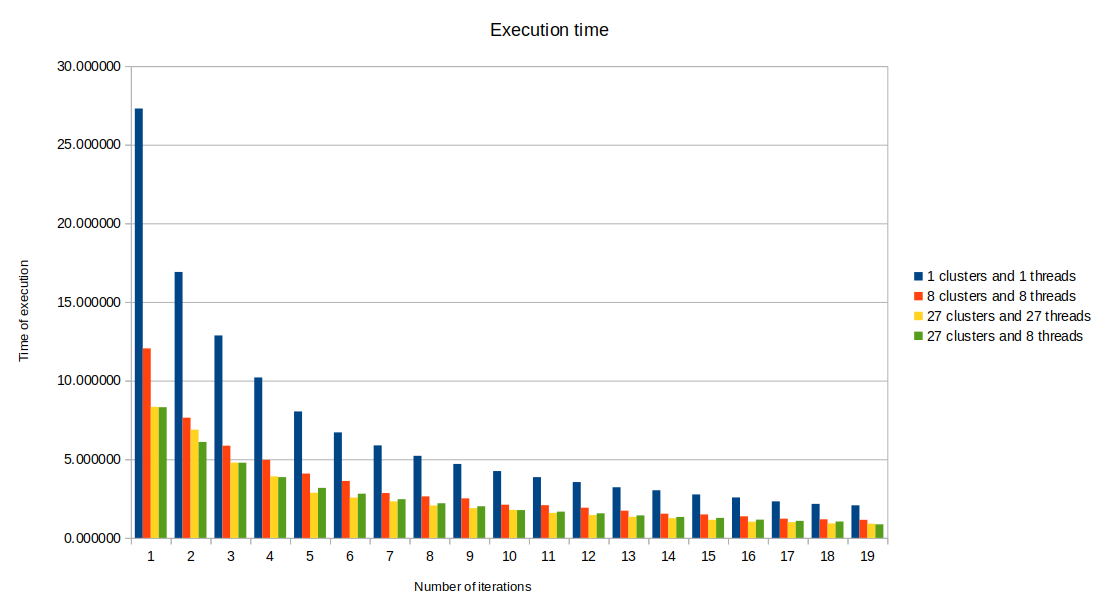
\includegraphics[width=18cm]{chart}
    \caption{Time of execution in seconds with different number of threads and clusters.}
    \label{fig:execution_time}
  \end{center}
\end{figure}

The Figure \ref{fig:execution_time} shows how much time does it take to simplify a mesh in one iteration. In total, there were 19 iterations to achieve the 85\% of simplification. The one iteration in this case is the full pass of the simplificaiton algorithm with waiting for all threads to finish processing. Naturally, the time is getting smaller with each iteration because we have less vertices to process. As we could expect, the single threaded version performs very poorly. Using more than 1 thread we can achieve better results with the best speedup around 3.5.

\begin{figure}[H]
  \begin{center}
    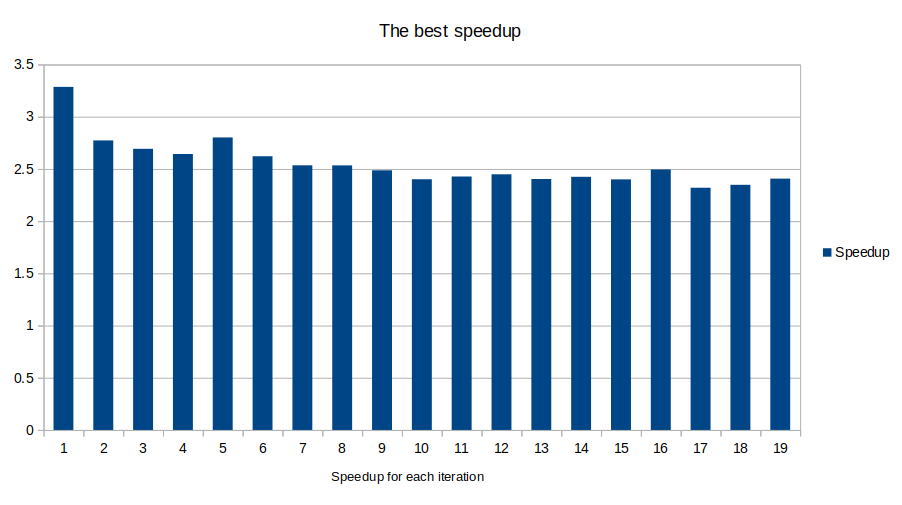
\includegraphics[width=16cm]{chart2}
    \caption{The best speedup for each iteration}
    \label{fig:speedup}
  \end{center}
\end{figure}

The Figure \ref{fig:speedup} desciribes the best speedup for each iteration from the tests in Figure \ref{fig:execution_time}. As you can see, the value oscillates around 2.5 and 3 which is a decent result for this complex algorithm. Moreover, in the Figure \ref{fig:execution_time} we can see Amdahl's law in practice. Incerasing number of threads does not improve speed up \cite{amdahl67}.

To avoid synchronization overhead I tried deep copies of a sub-meshes passed to processing threads. The problem with this solution is merging sub-meshes into the master mesh after simplification. To preserve local geometry on the edges the process of decemination need not to change or remove them. It gives a rise to another problem with convergence. Since, we cannot easily distinguish artificially created edges due to clustering between original edges, which we would like to simplify. Moreover, merging meshes takes time, so, at the end the algorithm does not gain much performance speedup.

Summarizing, the parallel execution of clusters gives a desired speedup. The algorithm is able to process big meshes up to a few million of faces in reasonable time, which is necessary for streaming purposes and a production usage.

\newpage
\section{Taubin Smoothing}

During my research and later implementation of the algorithm, I noticed faster convergance to selected level of reduction, if a mesh smoothing is used. For my purposes, I used Taubin Smoothing algorithm. The method is a linear low-pass filter that removes high curvature variations and does not produce shrinkage \cite{taubin95}. After the mesh is loaded to the program smoothing is done.

\begin{center}
  	\begin{table}[h!]
  	\begin{center}
  	\begin{tabular}{cc}
	\begin{subfigure}{1\textwidth}\centering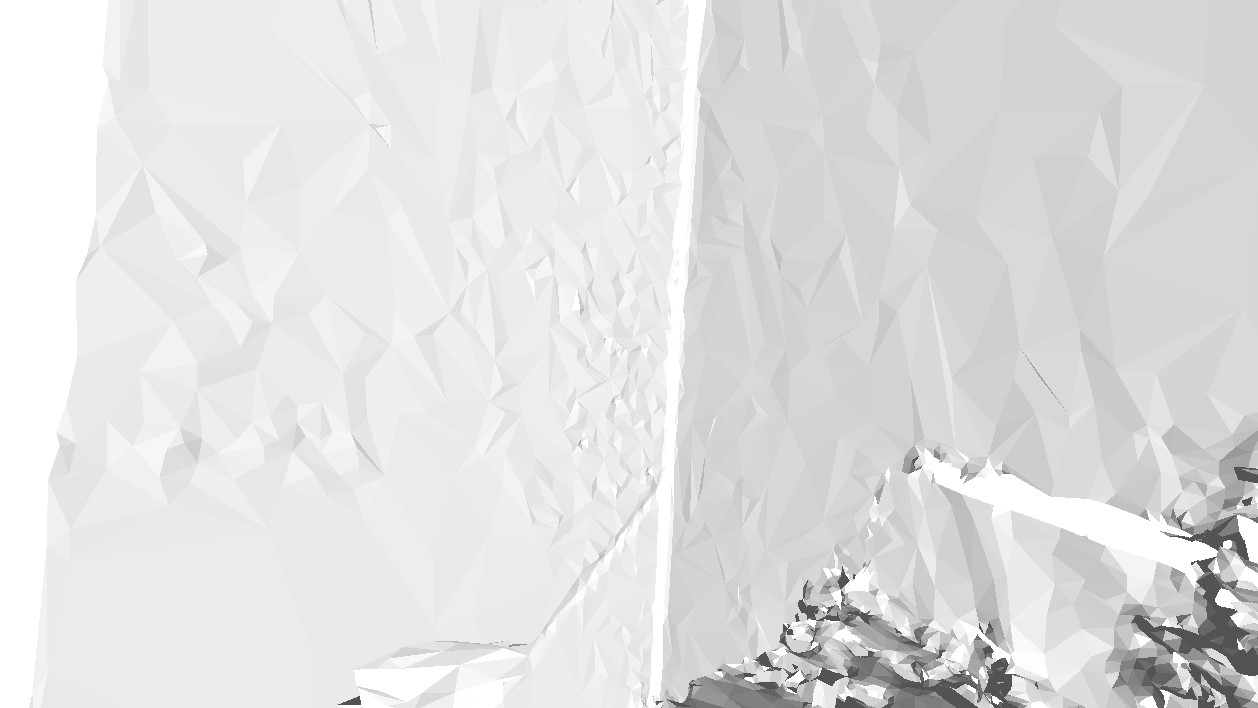
\includegraphics
		[width=0.8\columnwidth]{smooth}\caption{Simplification with smoothing}\label{smooth}\end{subfigure}\\
	\begin{subfigure}{1\textwidth}\centering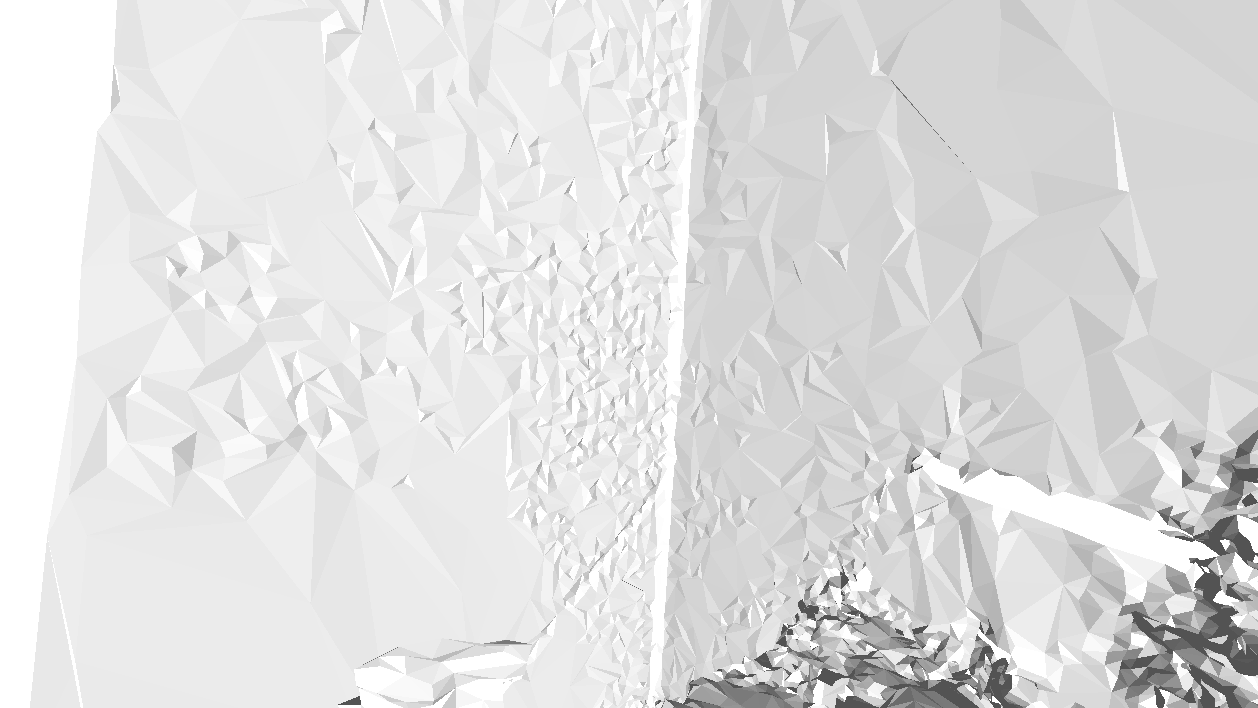
\includegraphics
		[width=0.8\columnwidth]{non_smooth}\caption{Simplification without smoothing}\label{non_smooth}\end{subfigure}
	\end{tabular}
	\caption{Comparision of the smoothing effect for 85\% simplification.}
  	\label{tab:smoothing_effect}
  	\end{center}
	\end{table}
\end{center}

\begin{table}[h!]
\centering
\begin{tabular}{ |c|c|c| } 
 \hline
 Iterations & Lambda & Mu\\
 \hline
 7 & 0.5 & -0.67\\ 
 \hline
\end{tabular}
\caption{Taubin algorithm parameters.}
\end{table}

The simplification was ran on the mesh with 396277 faces and 208825 vertices. The mesh was reduced to 50009 faces and 29347 vertices. In the Table \ref{fig:time_speedup} we can see that the speedup comapred with the single core is around 1.6. Additionaly in the Table \ref{tab:smoothing_effect} we can see that planar surfaces look better after simplification with smoothing.

\begin{table}[h!]
\centering
\begin{tabular}{ |c|c| } 
 \hline
 Time with smoothing & Time without smoothing\\
 \hline
 27.73 s & 43.06 s\\ 
 \hline
\end{tabular}
\caption{Taubin algorithm parameters.}
\label{fig:time_speedup}
\end{table}

\begin{figure}[h!]
  \begin{center}
    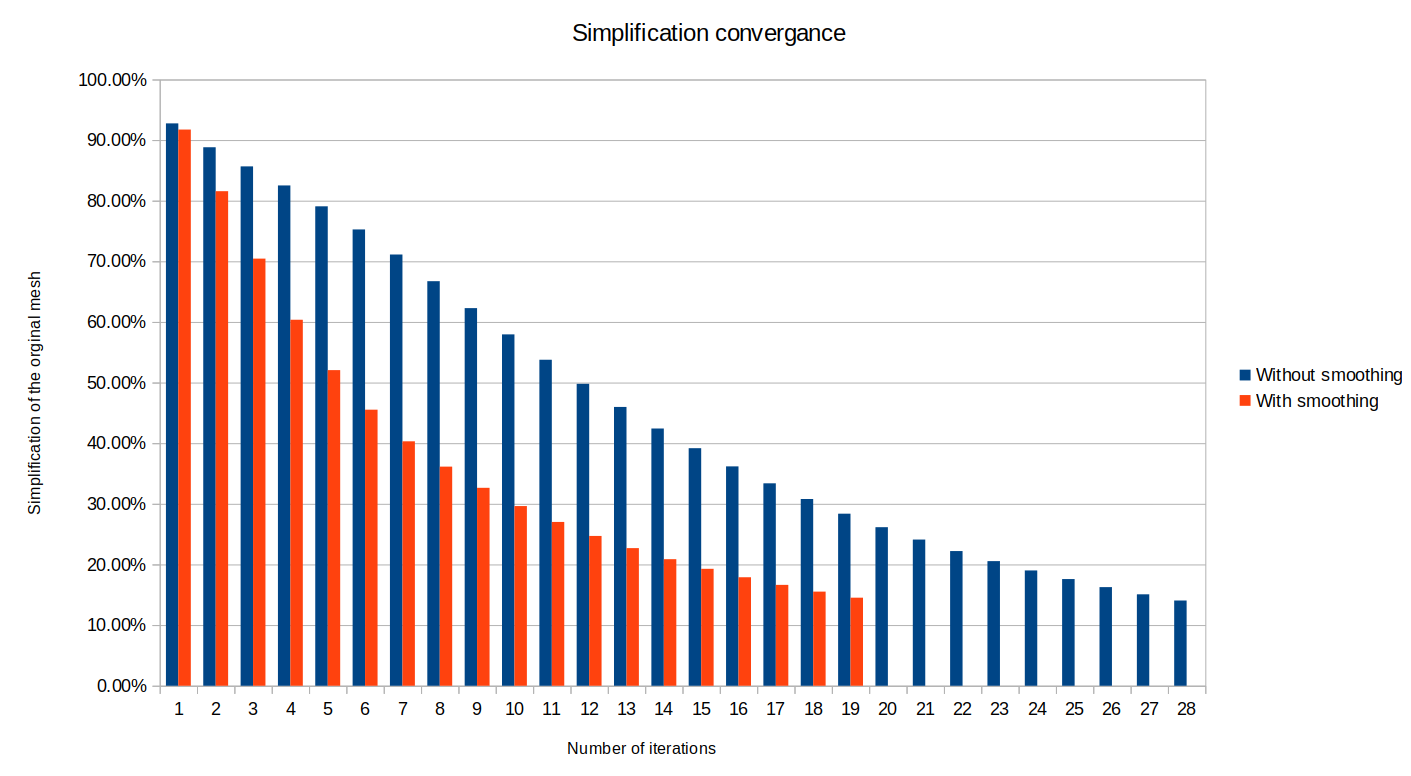
\includegraphics[width=16cm]{convergance}
    \caption{Convergance to 15\% of the original mesh.}
    \label{fig:convergance}
  \end{center}
\end{figure}

Figure \ref{fig:convergance} shows that with smoothing the convergance takes only 19 full iterations, whereas for a regular version it takes 28. It means that with a small overhead, the complexity of Taubin's algorithm is linear $O(n)$ \cite{taubin95}, we can gain better quality of the simplified mesh and additional speedup.

\newpage
\section{Summary of the Algorithm}

\begin{enumerate}
\item Smooth mesh using Taubin algorithm (optional).
\item Cluster the mesh:
\begin{enumerate}
\item Split the mesh according to number of selected clusters; for example 2x2x2=8.
\item Add a task for each cluster to the queue.
\end{enumerate}
\item Wait for all threads from the threadpool to finish processing simplification algorithm [QSlim] ran on all clusters. Each thread does:
\begin{enumerate}
\item Build the heap with edges.
\item Deceminate edges till reaching the threshold level.
\end{enumerate}
\item Update the mesh structure:
\begin{enumerate}
\item Remove faces flagged as invalid.
\item Reset properties for each remaining face and vertex.
\end{enumerate}
\item Repeat from the second step till convergance.
\end{enumerate}

As you can see above, the parallel algorithm nicely wraps Garland's algorithm in the third step. We repeat the whole procedure from the second step till either reduction level is reached, or the number of iterations is exceeded. To achieve a nice planar simplification the adaptive threshold level is used. The third step is terminated for a thread if the cost level is higher than the threshold.

\newpage
\section{Comparison to Commercially Available Products}

Most of commercially available algorithms use only geometry to generate an approximation of a mesh. Moreover, libraries like OpenMesh do not provide an API to use all attributes of a vertex. We can add more constraints to our optimization objective, but they are not solved jointly like in my case. Additionally, those algorithms simplify a mesh globally which introduces almost even decemination for all surfaces. Below I present comparison of my method with serveral different approaches where the goal was to reduce the original mesh 85\%.

\begin{figure}[H]
  \begin{center}
    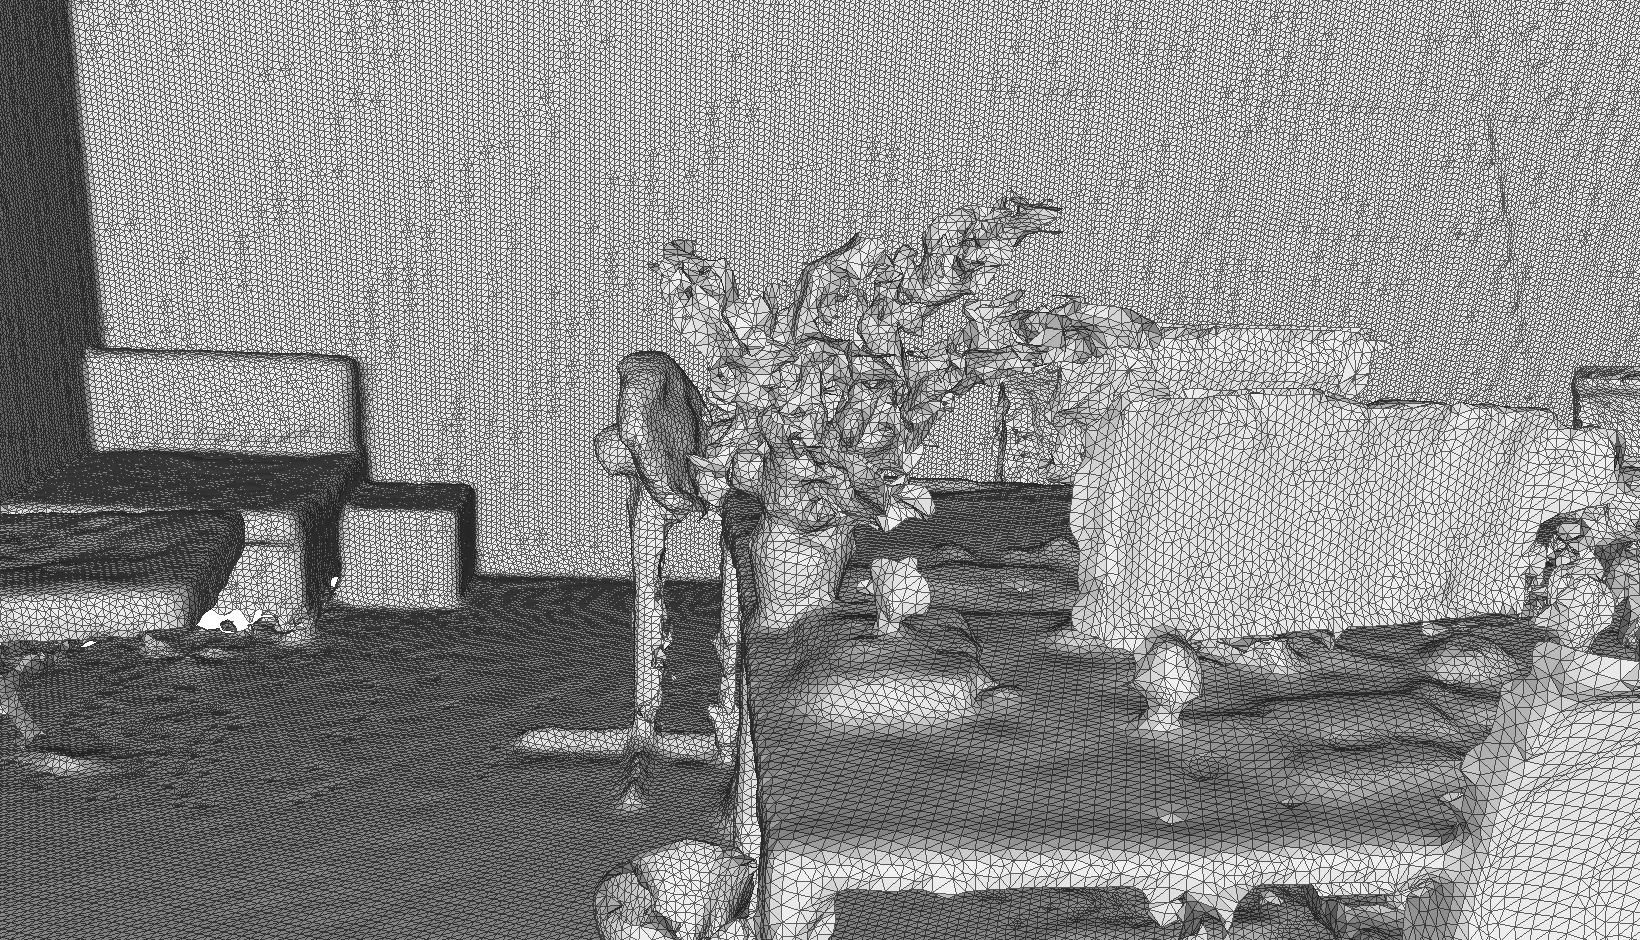
\includegraphics[width=16cm]{original}
    \caption{The original mesh.}
    \label{fig:original}
  \end{center}
\end{figure}

Figure \ref{fig:original} shows the original mesh with evenly distributed faces. We can see that the amount of faces used for the wall is unecessary. Therefore, we can successfully apply simplification to this surface.

\begin{figure}[H]
  \begin{center}
    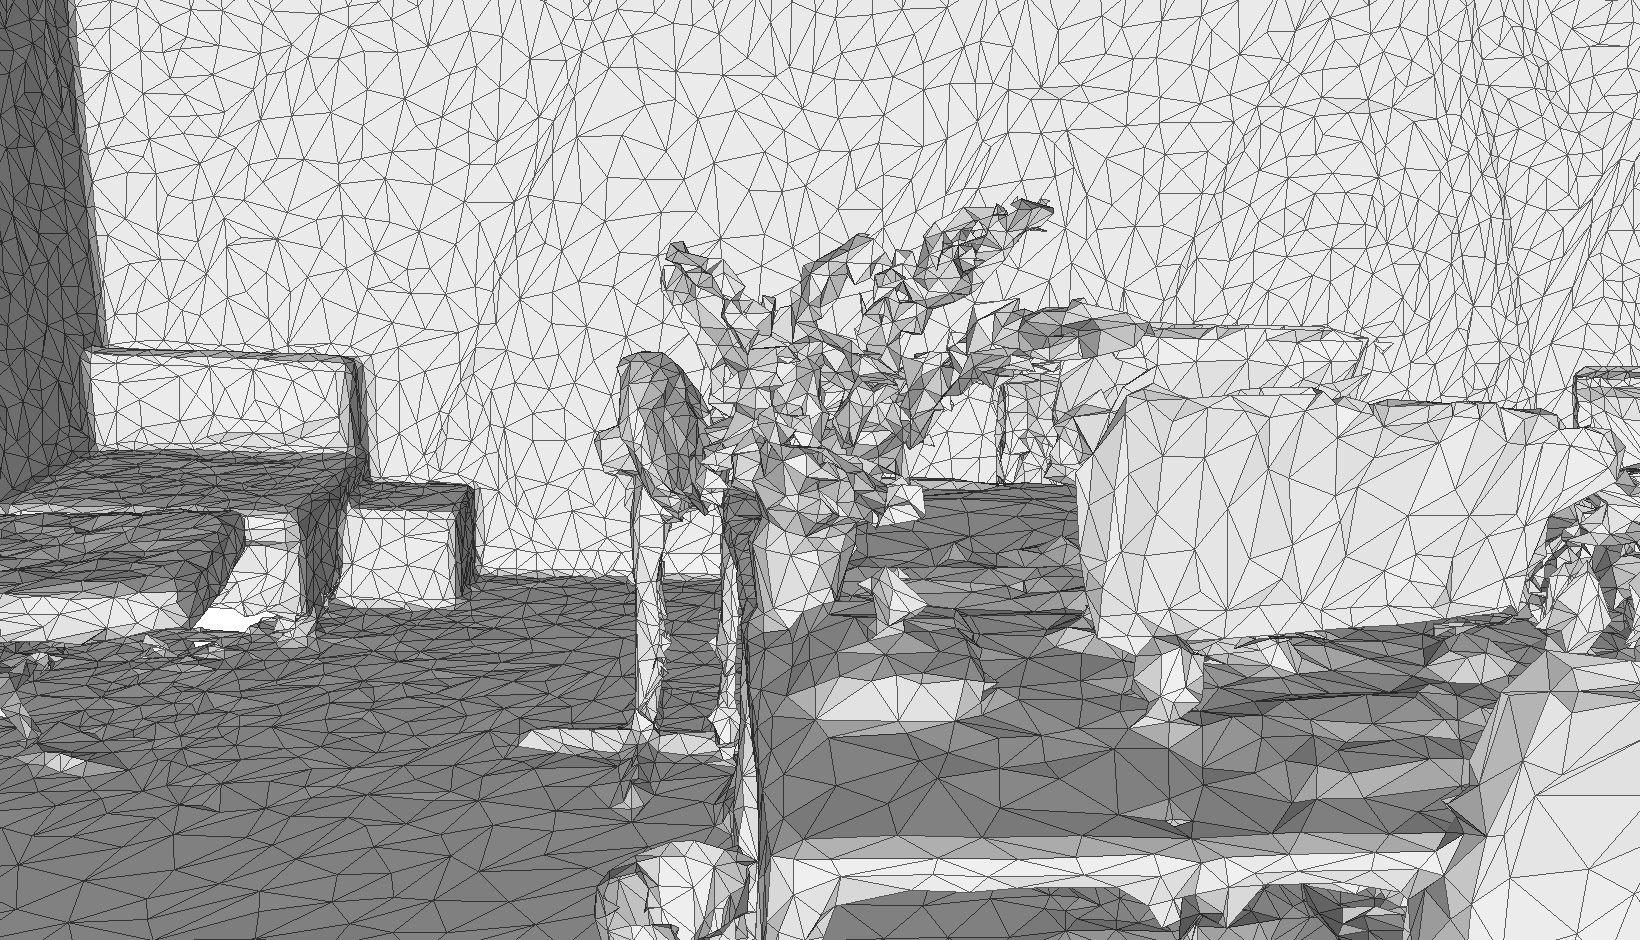
\includegraphics[width=16cm]{fast_collapse}
    \caption{Fast-Quadric-Mesh-Simplification algorithm.}
    \label{fig:fast_collapse}
  \end{center}
\end{figure}

Figure \ref{fig:fast_collapse} shows Fast-Quadric-Mesh-Simplification algorithm by Sven Forstmann, which is \href{https://github.com/sp4cerat/Fast-Quadric-Mesh-Simplification}{a github implementation} of memory efficient and very fast edge collapse mesh simplification method. According to the creator its around 4 times faster than Meshlab version. Figure \ref{fig:fast_collapse} shows the result where you can see that all surfaces are deceminated evenly. Moreover, the algorithm is based only on vertex iteration with adaptive thresholding without bulding a heap of edges.

\begin{figure}[H]
  \begin{center}
    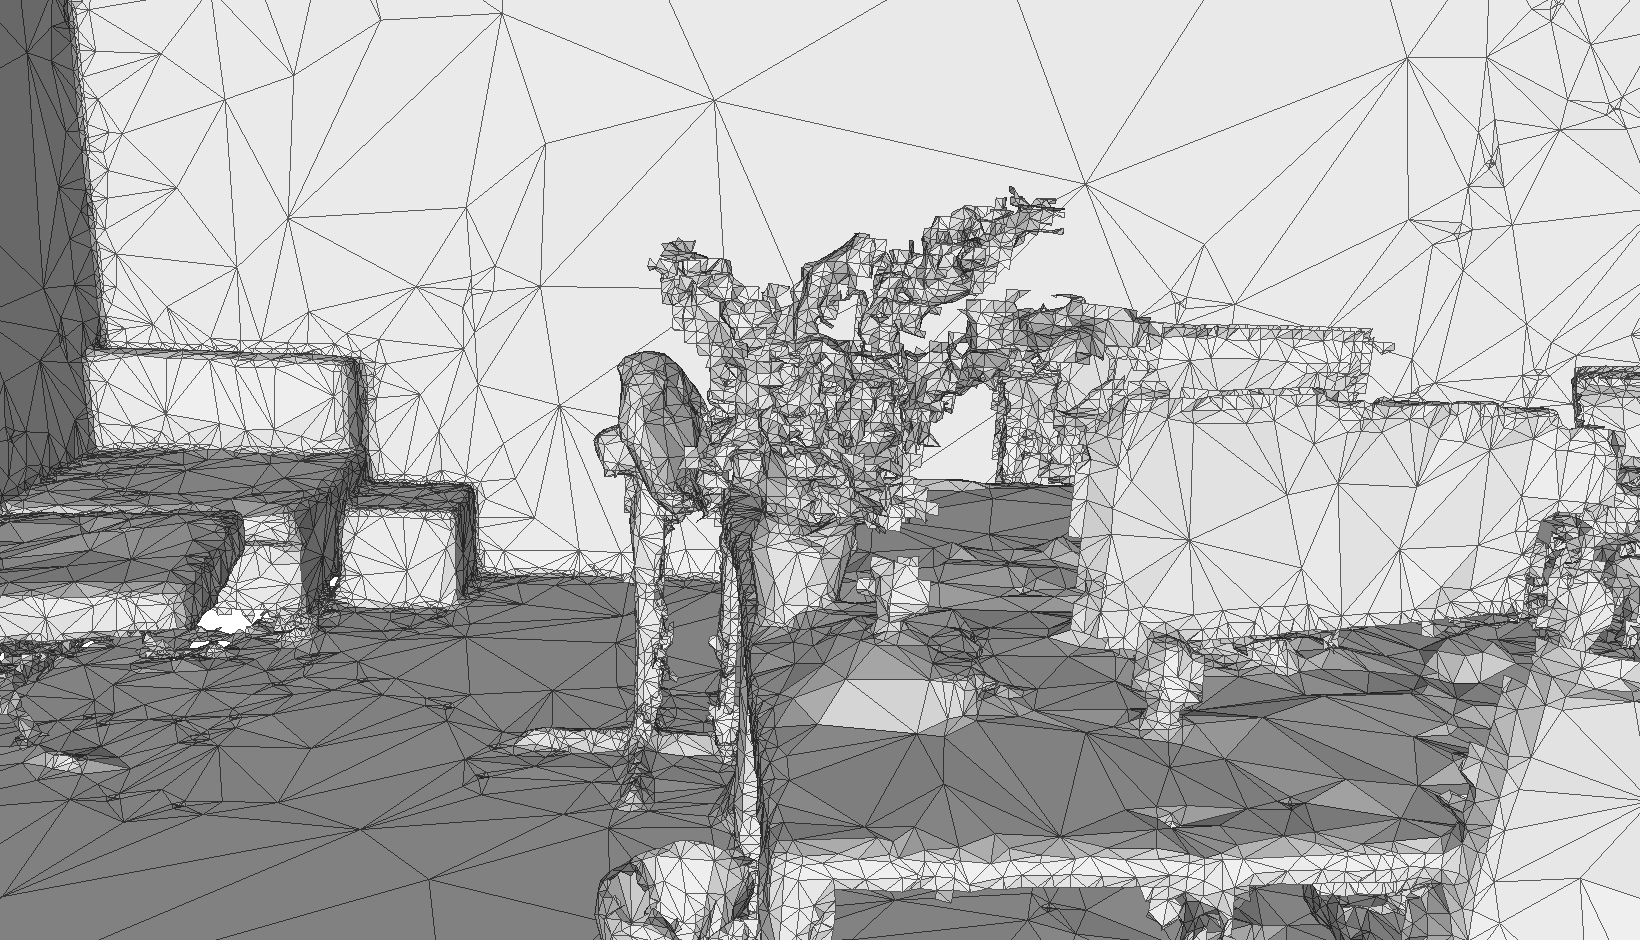
\includegraphics[width=16cm]{open_mesh}
    \caption{OpenMesh with geometry and normals.}
    \label{fig:open_mesh}
  \end{center}
\end{figure}

Figure \ref{fig:open_mesh} shows the usage of OpenMesh library, where the decemination was done using geometry and normals. Because of that, border edges were not touched. In this case, borders can produce errors in the approximation, like spiky edges. Border preserving is mostly visible on the plant structure or the monitors edges. This method gives the poorest result, however, it is almost as fast as Fast-Quadric-Mesh-Simplification.

\begin{figure}[H]
  \begin{center}
    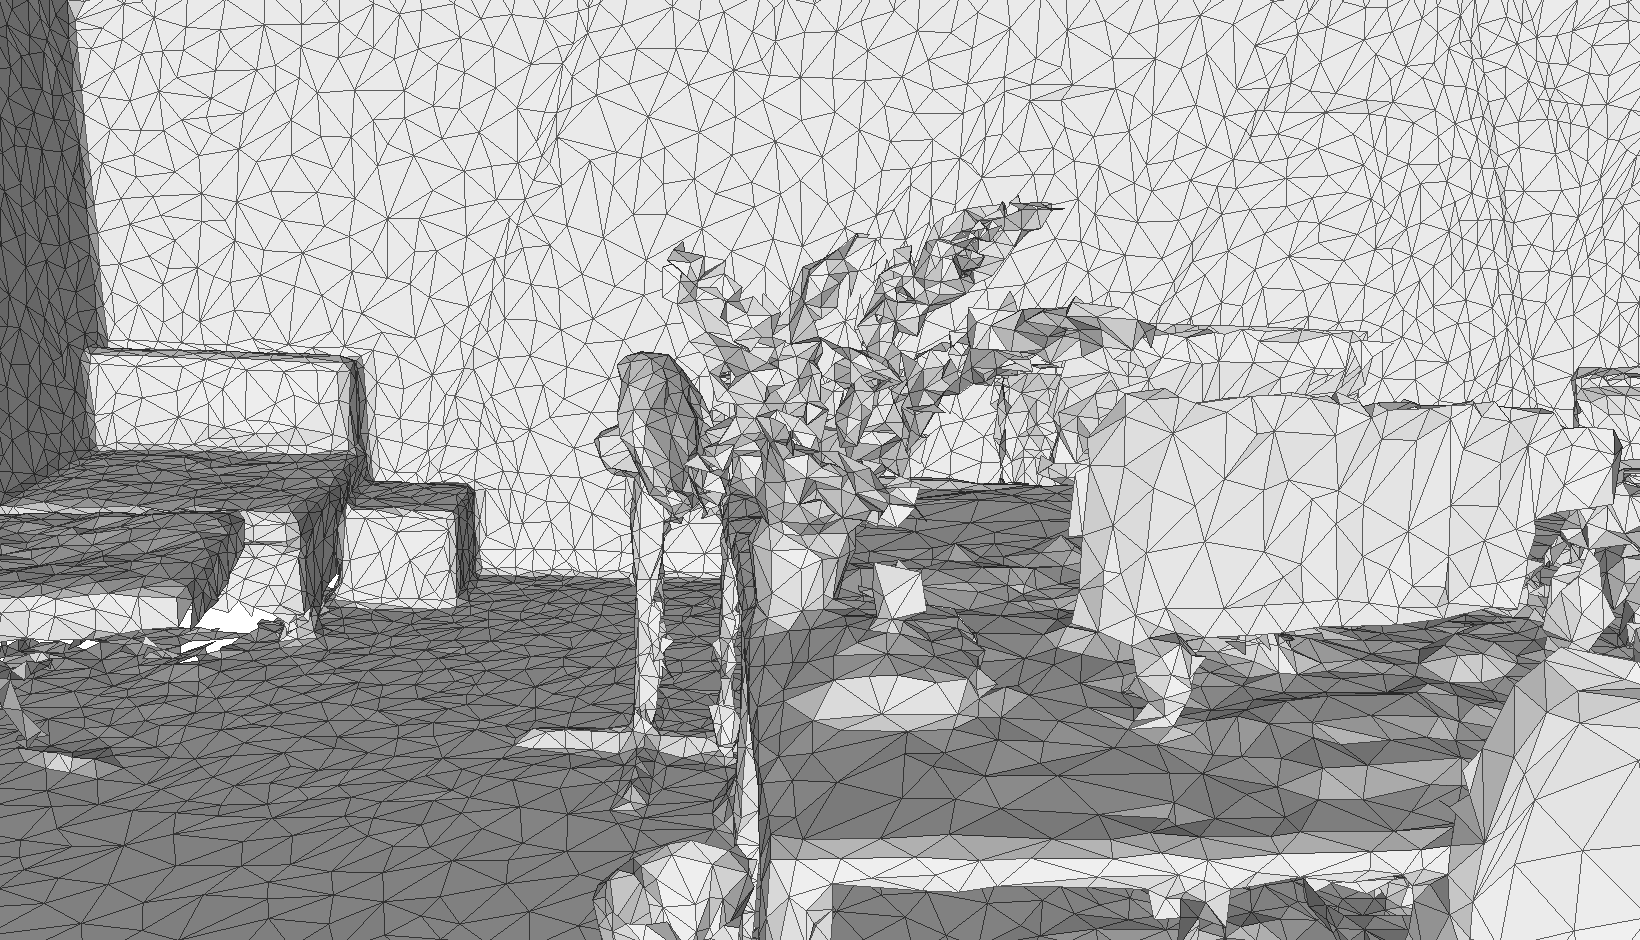
\includegraphics[width=16cm]{mesh_lab}
    \caption{MeshLab version of simplification.}
    \label{fig:mesh_lab}
  \end{center}
\end{figure}

As you can see in the Frigure \ref{fig:mesh_lab} the approximation is very similar to Figure \ref{fig:fast_collapse}. However, the MeshLab version is slower than Fast-Quadric-Mesh-Simplification algorithm.

\begin{figure}[H]
  \begin{center}
    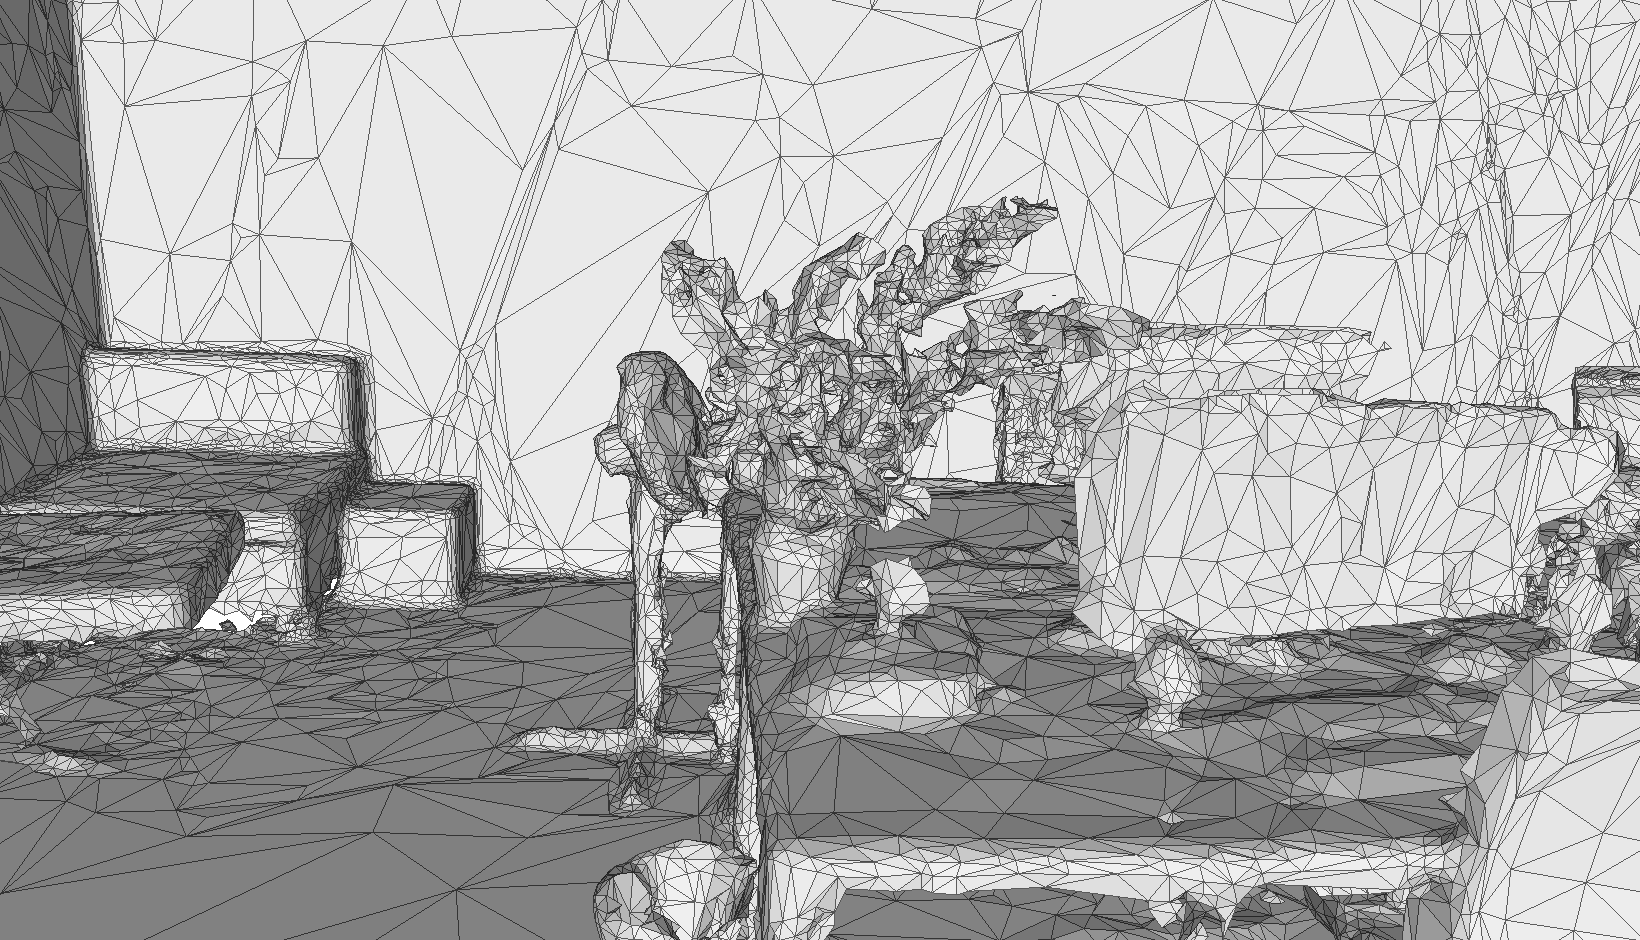
\includegraphics[width=16cm]{my_3}
    \caption{Parallel QSlim with adaptive thresholding algorithm using only geometry.}
    \label{fig:my_3}
  \end{center}
\end{figure}

Figure \ref{fig:my_3} shows approximation produced by my version of the algorithm. The complex shapes are preserved much better than in all previous versions. However, there is still room for even more aggressive decemination of planar surfaces. To achieve it, we need to use more attributes in our joint optimization.

\begin{figure}[H]
  \begin{center}
    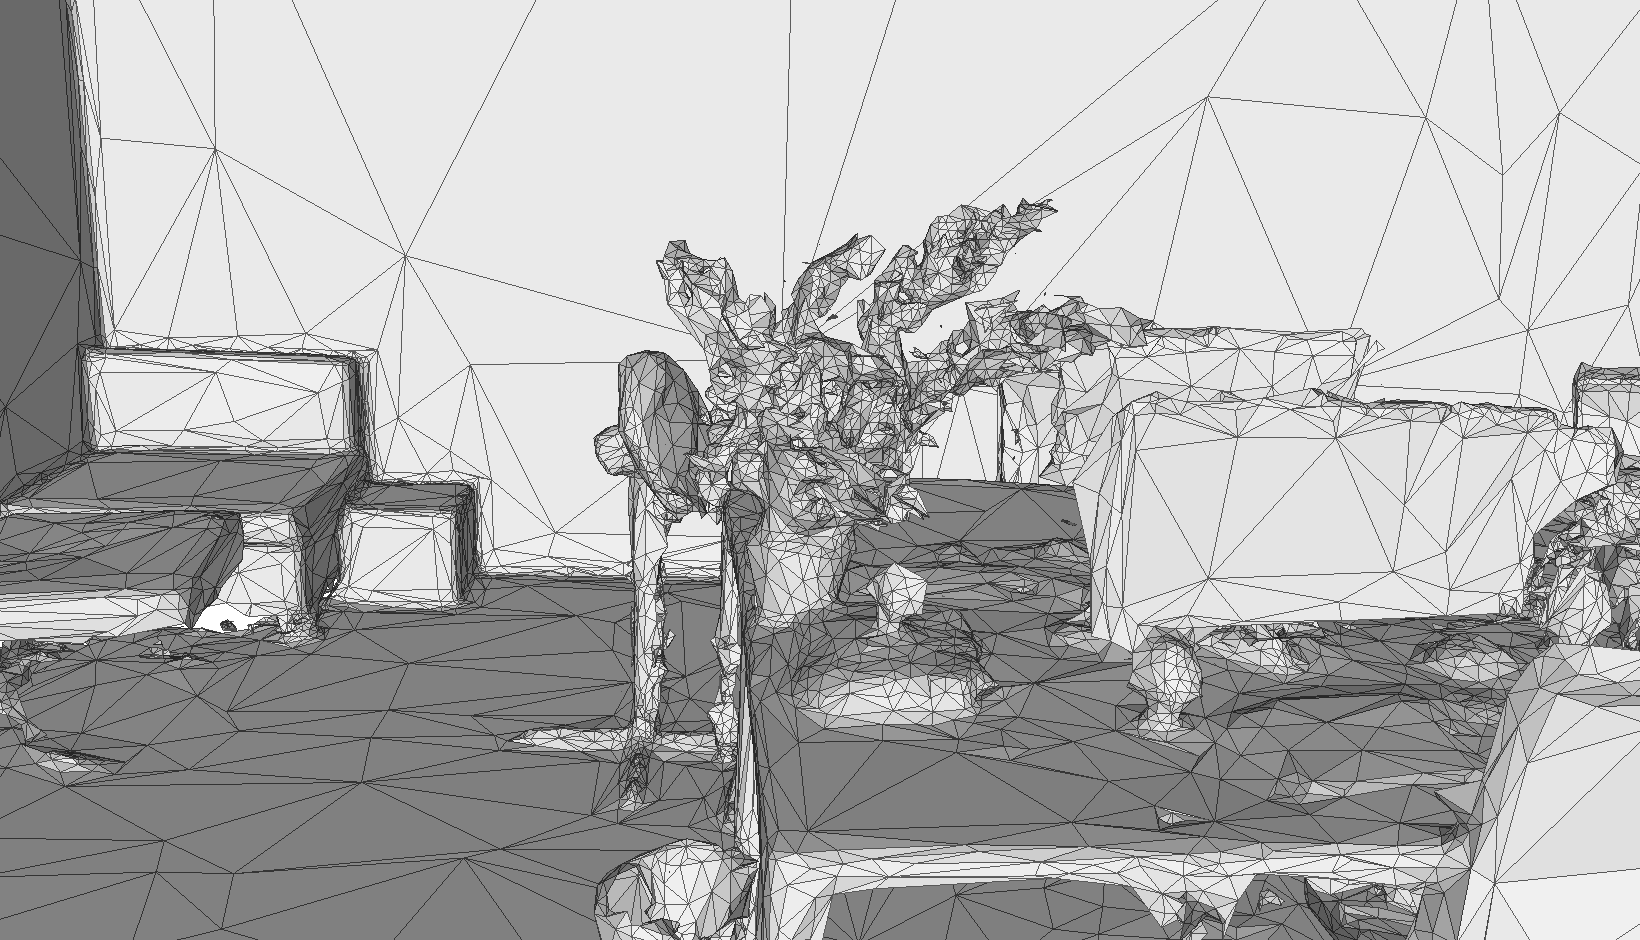
\includegraphics[width=16cm]{my_9}
    \caption{Parallel QSlim with adaptive thresholding algorithm using geometry, color and normals.}
    \label{fig:my_9}
  \end{center}
\end{figure}

Figure \ref{fig:my_9} shows the best approximation under the constrain of deceminating most of the planar surface. All complex shapes are almost intacted from the original mesh. The faces which describe the wall are as big as possible. Moreover, iterative nature of the algorithm, allows to level small surfaces elevation changes. For instance, the interior part of the pouf near the wall. In the Figure \ref{fig:my_3} we can see that the noise and level changes, prevented this region from being simplified. In the version with all attributes $[geometry, normal, color]$, the interior part is nicely leveled.

\begin{figure}[H]
  \begin{center}
    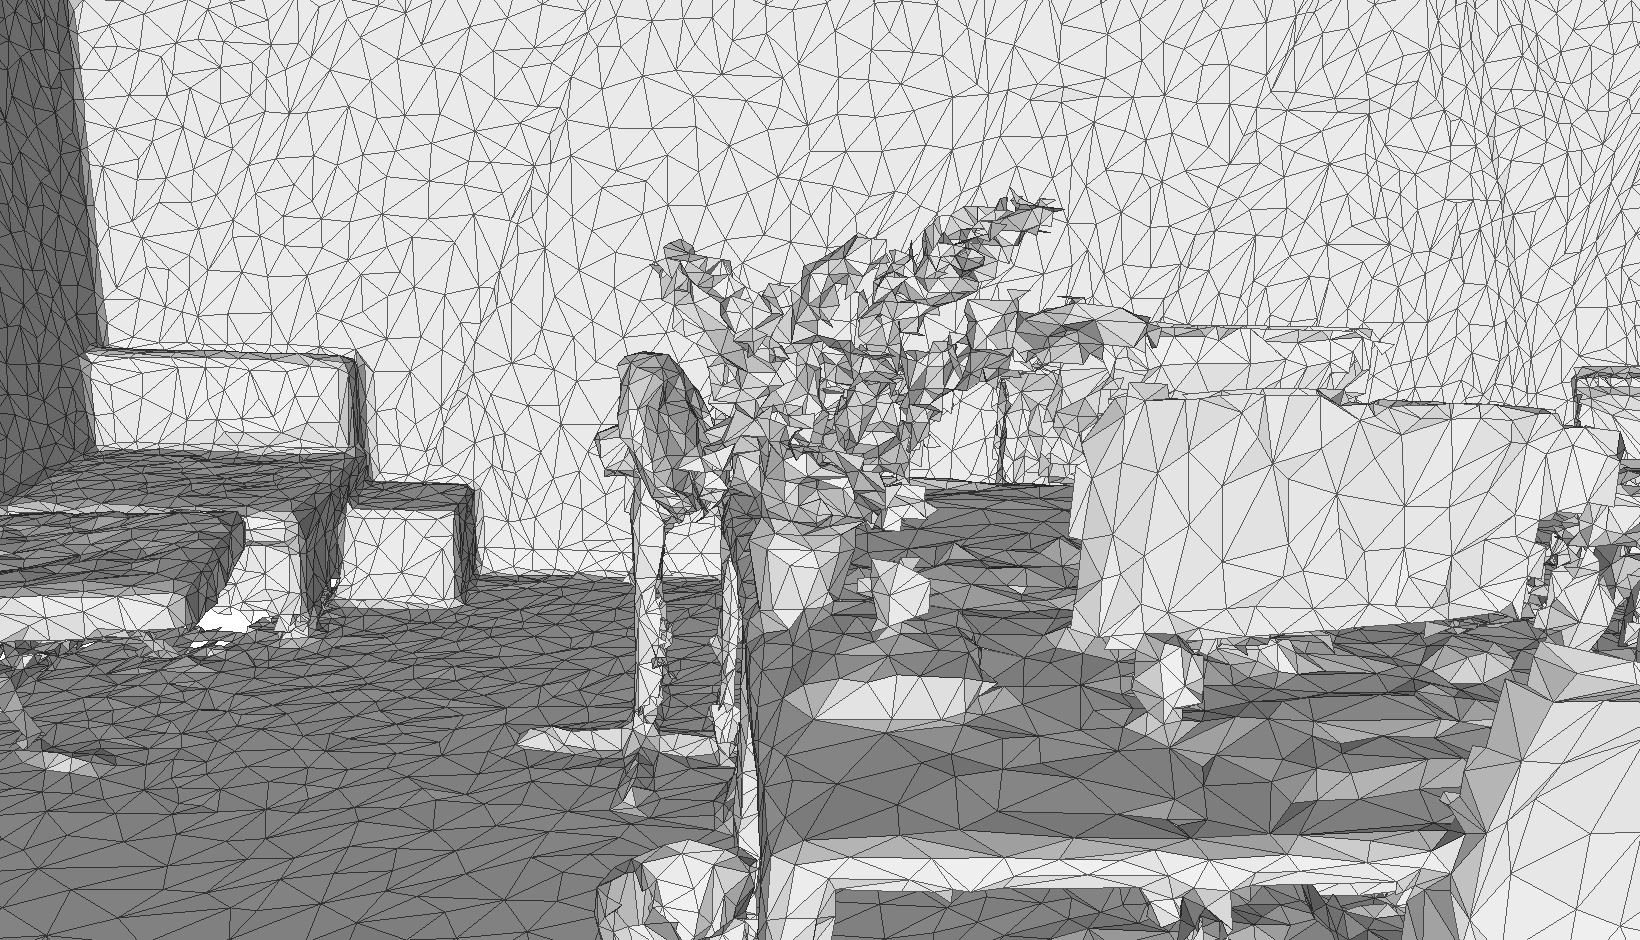
\includegraphics[width=16cm]{rapid_compact}
    \caption{RapidCompact version of simplification.}
    \label{fig:rapid_compact}
  \end{center}
\end{figure}

For the completeness, I used for the comparison a paid version of the algorithm done by RapidCompact. However, the result is almost exactly the same like in the case of the MeshLab and Fast-Quadric-Mesh-Simplification algorithm.
